%=================================================================================
%                西南交通大学研究生学位论文LaTeX模板
%=================================================================================

% 使用全局样式swjtuThesis,大部分的模板格式均在样式文件中定义完成
\documentclass[oneside,openany]{swjtuThesis}

% 超链接颜色设置(调试时候使用,方便区分文本和超链接)
\hypersetup{colorlinks,linkcolor=red,citecolor=green,urlcolor=magenta}

% 加载信息
%---------------------------------------------------------------------------------
%                西南交通大学研究生学位论文基本信息
%---------------------------------------------------------------------------------

% 论文信息
% 定义申请学位
% 请注意:博士学位候选人输入 Doctor,硕士学位候选人输入 Master
\def\degree{Master} 

% 论文中文标题
% 请注意:标题控制在36个汉字以内),其中用 \\ 实现标题换行,单行不得超过18个汉字。
% 		  \underline命令用于实现标题的下划线,请把标题输入在\underline命令的的{}中
\cTitle{\underline{面向无线网络的新型传输层} \\ \underline{协议设计与实现}}

% 论文英文标题(72个字符以内,包含空格)
\eTitle{Design and Implementation of New Transport Layer Protocol for Wireless Networks}


% 国内图书分类号
\CI{TM30}
% 国际图书分类号
\UDC{621.3}
% 保密等级
\secLevel{公开}

%----------------------------
% 学生信息
% 中英文姓名
\author{董泽锋}
\eAuthor{Dong Zefeng}

% 年级
\grade{2014}

% 学科(工学、理学、社会学,etc)
\cDiscipline{工学}
\eDiscipline{Engineering}

% 专业(10个汉字以内)
% 请注意:对于超过10个汉字的专业,比如“防灾减灾工程及防护工程”,目前排版仍然不够美观,正在修正。
%        也请相应专业的同学提供过往师兄的硕士论文以供参考。
\cMajor{通信与信息系统}
\eMajor{Communication and Information System}

% 导师(10个汉字以内)
% 请注意:导师姓名和导师的职称之间加上\hspace{0.1em}以增大间距,整体显得更为美观。 
\cTutor{陈庆春 \hspace{0.1em} 教授/博导}
\eTutor{Prof. Chen Qingchun}

% 封面日期,依次为年,月,日
\cDate{二〇一七}{四}{十三}
\eDate{2017}{April}{13}				% 加载论文信息
%---------------------------------------------------------------------------------
%                判断学位论文类型(硕士学位or博士学位)
%---------------------------------------------------------------------------------

% 请注意:本文件已经定义好需要使用的字符串,不建议用户更改。

\newif\ifdegreedoctor
\newif\ifdegreemaster

\def\temp{Doctor}
\ifx\temp\degree
\degreedoctortrue  \degreemasterfalse
\fi

\def\temp{Master}
\ifx\temp\degree
\degreedoctorfalse  \degreemastertrue
\fi

\ifdegreedoctor
\newcommand{\cDegree}{博士}
\newcommand{\eDegree}{Doctor of }
\fi

\ifdegreemaster
\newcommand{\cDegree}{硕士}
\newcommand{\eDegree}{Master of }
\fi    			% 区分硕博类型(模板自动区分)
%---------------------------------------------------------------------------------
%                学位论文LaTeX模板使用宏包文件
%---------------------------------------------------------------------------------

% 数学公式常用宏包(实现更多样的数学公式输入)
\usepackage{amsmath}
\newtheorem{myDef}{\hspace{2em}定义}[chapter]
\usepackage{mathtools}
\usepackage{wasysym}

\makeatletter  
\newif\if@restonecol  
\makeatother  
\let\algorithm\relax  
\let\endalgorithm\relax  
\usepackage[linesnumbered,ruled,vlined]{algorithm2e}%[ruled,vlined]{  
\usepackage{algpseudocode}  
\usepackage{amsmath}  
\renewcommand{\algorithmicrequire}{\textbf{Input:}}  % Use Input in the format of Algorithm  
\renewcommand{\algorithmicensure}{\textbf{Output:}} % Use Output in the format of Algorithm   
%\newcommand{\algorithmicbreak}{\textbf{break}}
\newcommand{\Break}{\textbf{break}}
\newcommand{\Retuan}{\textbf{return}}
\usepackage{algorithmicx}

\usepackage{colortbl}
%\usepackage{algorithm}  
%\usepackage{algpseudocode}  
%\usepackage{amsmath}  
%\renewcommand{\algorithmicrequire}{\textbf{Input:}}  % Use Input in the format of Algorithm  
%\renewcommand{\algorithmicensure}{\textbf{Output:}} % Use Output in the format of Algorithm 

\usepackage{listings}
\usepackage{xcolor}
\lstset{
	basicstyle=\ttfamily,
	numbers=left, 
	%numberstyle=\tiny, 
	keywordstyle=\color{blue!70},  
	commentstyle=\color{red!50!green!50!blue!50}, 
	frame=shadowbox, 
	rulesepcolor=\color{red!20!green!20!blue!20},
	tabsize=4,breaklines 
}
%\lstset{
%	basicstyle=\ttfamily,
%	numbers=left,
%	keywordsstyle=\color[RGB]{0,0,255},
%	commentstyle=\color[RGB]{0,128,0}
%	frame=shadowbox,
%	rulesepcolor=\color{red!20!green!20!blue!20},
%	showspaces=false,
%	showstringspaces=false,
%	showtabs=false,
%	tabsize=4,breaklines
%}


\usepackage{booktabs}
\usepackage{threeparttable}
\usepackage{amssymb}

\usepackage{amsfonts}
% 表格制作常用宏包(实现更多表格功能,比如不等线粗的三线表)
\usepackage{multirow}
\usepackage{booktabs}

% 插入图片常用宏包(实现多种格式的调用)
\usepackage{graphicx}

% 图表题注格式宏包(实现《规范》要求的题注格式)
\usepackage{caption}
\captionsetup{labelformat=simple, labelsep=space, font=bf}

% TeX系列标识的正确输入宏包(实现正确插入TeX相关的字符串)
\usepackage{dtklogos}

% 列表制作常用宏包(用于调用小间距列表)
\usepackage{paralist}
\usepackage{tabularx}
\usepackage{array}
% 外框宏包
\usepackage{framed}
\usepackage{rotating}
\usepackage{url}

% 引用文献实[Ni-Ni+j]的宏包
\usepackage{cite}

% 使用列表时要用到的包
\usepackage{enumitem}
% 英文采用Times New Rome字体(建议把这个宏包放在最后避免发生宏包冲突)
\usepackage{fontspec}
\setmainfont{Times New Roman}			% 加载使用宏包


\begin{document}

%---------------------------------------------------------------------------------
% 封面生成(包括中、英文封面、版权协议以及硕(博)士主要工作简述)
\makecover

% 论文前言(包括中、英文摘要及目录,页码为罗马数字,在研究生论文目录中不显示摘要)
\frontmatter
\pagenumbering{Roman}
\thesispagestyle{-4}{西南交通大学\cDegree{}研究生学位论文}{第~\thepage~页}	% 页眉设置

% 加载中文摘要
%---------------------------------------------------------------------------------
%                西南交通大学研究生学位论文:中文摘要
%---------------------------------------------------------------------------------
% 中文摘要输入区
\cabstract
{
	%%写完对照摘要要求,看是否合适
	%%可以写本文的主要工作包括。。。。
	无人机一般工作在室外空域,
	具有移动性高的特点,
	这决定了其经常面临大尺度衰落信道环境,
	数据链路错包、丢包频繁。
	因此,基于传输层协议( TCP ) 的无人机视频传输面临着吞吐率受限、时延较大的问题。
	这一问题很大程度上又是因为TCP协议本身的设计导致的。
	\par
	TCP将丢包看做是链路出现拥塞的标志,
	然后启动相应的拥塞控制算法,
	降低传输速率。
	考虑到有线网络中极低的误码率、拥塞是丢包的主要原因,
	这一机制是适用的。
	然而对于无人机来说,
	由于天气、障碍物、多径干扰等各种因素,
	TCP丢包率比在有线网络中大得多,
	且丢包多由遮挡、传输错误导致。
	传统TCP无法鉴别拥塞丢包和非拥塞丢包,
	不分区别地频繁启动拥塞控制算法,
	降低数据发送速率,
	将导致TCP无法充分利用可用带宽,
	减小无人机视频传输的速率,
	提高传输时延。
	有必要改进标准TCP协议以提高基于TCP协议的无人机视频传输的性能。
	网络编码的出现对于解决这一问题给出了一个思路。
	通过在发送端冗余编码,
	可以一定程度掩盖链路中出现的丢包,
	从而提高数据传输的速度,
	降低时延。
	\par
	本文分析了基于TCP协议的无人机视频传输所面临的问题,
	并指出问题核心是TCP协议在面对lossy信道时的低效。
	对近些年来改善lossy信道中TCP性能的相关工作进行了梳理。
	介绍了网络编码原理,
	尤其是随机线性网络编码。
	对于batch-coding和pipeline-coding进行了比较,
	结合无人机视频传输应用场景,
	分析了其优缺点。
	在以上基础上,
	设计实现了流水线编码TCP协议,
	并将其移植入嵌入式设备。
	在模拟丢包网络中,
	对流水线编码TCP进行性能测试,
	与TCP-Reno协议进行性能对比,
	分析影响其性能的关键因素。
	在了解流水线编码TCP协议不足的情形下,
	对其做了进一步改进,
	以更好地适应无人机视频传输应用场景。
	提出了前向重传机制以应对一个RTO内的突发丢包;
	提出了一种新的自适应冗余度算法以应对网络的变化;
	对冗余包的发送时机给出改进以降低平均解码时延;
	设计补偿重传机制以降低解码端解码矩阵维度和减小解码时延;
	改进编码系数的设定以降低首部开销。
	最后,本文搭建了无人机视频传输实验平台,
	验证改进后的编码TCP协议对无人机视频传输性能的提高。
	\par
	
}
{无人机视频传输;传输层协议;编码;重传;自适应冗余;丢包} 	% 中文关键词输入区,关键词之间用“;”分开,不超过五个

% 加载英文摘要
%---------------------------------------------------------------------------------
%                西南交通大学研究生学位论文:英文摘要
%---------------------------------------------------------------------------------

% 英文摘要输入区
\eabstract
{
Here is for you to write the English abstract.



}
{Network Coding; Transport Protocol; Retransmission ; Adaptive Redundancy; Packet Loss}	% 英文关键词输入区,关键词之间用“; ”分开,不超过五个

% 目录生成
\tableofcontents

%---------------------------------------------------------------------------------
% 学位论文正文(包含各章节内容和结论,页码为阿拉伯数字)
\mainmatter
\thesispagestyle{-4}{西南交通大学\cDegree{}研究生学位论文}{第~\thepage~页}	% 页眉设置

% 加载论文正文(第1章 - 第N章、结论)
% 目前共有四个章节文件,用户可以自行在content/:文件夹中添加chap0X.tex文件
%---------------------------------------------------------------------------------
%                西南交通大学研究生学位论文:第一章内容
%---------------------------------------------------------------------------------

\chapter{绪论}
\par
本章首先介绍无人机视频传输的广泛应用及其现有的技术方案,
分析各自的优缺点。
对WIFI机制下的无人机视频传输所依赖的TCP协议进行了粗略的描述。
分析基于TCP协议的无人机视频传输所面临的问题,
指出问题核心乃是TCP协议本身的丢包模型设计。
重点指出了TCP协议的拥塞控制在lossy信道下的劣势及对无人机视频传输的影响。
阐述了改进TCP协议的必要性,
对国内外学者在改进lossy信道环境下TCP性能的研究现状进行分析和比较。
最后介绍了本论文的工作及论文的相关安排。
\section{论文的研究背景和意义}
\par
近几年,
得益于集成电路技术、通讯技术的飞速发展,
无人机开始进入民用市场,
其成为一种大众消费品的趋势越来越明显。
以大疆为代表的国内无人机产业快速发展并占据世界领先地位。
无人机航拍也逐渐成为了普通人都可以应用的一项技术。
无人机航拍技术方案主要分为两类:
第一种是类似DJI Lightbridge\footnote{关于DJI Lightbridge,参见\url{http://www.dji.com/cn/dji-lightbridge}}的专有数据链技术,
包含数字图传和模拟图传,
其优点是传输时延小和单向广播;
第二种是基于现有TCP/IP网络协议体系下的视频传输技术,如WIFI图传。
其缺点是传输时延比较大,
容易受到无线链路中的各种干扰。
WIFI图传虽然性能一般,
但是价格低廉,
无需专门的操控设备,
在低价民用市场仍然具有一定市场份额。
\par
WIFI机制下,
每个数据包必须完整无误传输,
一旦数据错误或有丢失,
就需要重新发送,
一般都是基于TCP协议来进行图传。
在TCP协议中,
每个TCP报文都有一个序号,
只有接收端按序收到正确的报文,
发送端才会收到接收端回复的相应报文的确认( Acknowledgement,ACK )。
另一方面,
丢包或者乱序包表明传输出错。
ACK机制保证了TCP的可靠传输,
但当丢包发生时,
由于需要反馈或者超时才能进行重传,
会显著增大无人机视频传输的时延。
\par
TCP-Reno是目前应用最为广泛的TCP协议之一。
它有四个传输阶段:
慢启动,拥塞避免,快恢复和快重传。
TCP维护了两个变量,拥塞窗口大小( cwnd)和慢启动门限( ssthresh)。 
cwnd的初始值设为最大报文段大小( MSS)。
一个TCP连接建立起来后,
首先进入慢启动阶段。
对于每一个ACK,
cwnd增长一个MSS大小;
因此,cwnd随着往返时延( Round-Trip Times,RTT)进行指数增长。
当cwnd超过了ssthresh,
TCP发送端进入拥塞避免阶段。
当发送窗口内所有的报文都被确认后,
cwnd才会增长一个MSS大小,
也就是说cwnd随着RTT线性增长。
如果传输链路中的某个节点因为拥塞而导致了丢包,
或者发送端收到3个重复ACK,
或者发送端的重传定时器超时,
发送端都会减小cwnd的值,
进而减小发送速度,
以便缓解链路的拥塞状况。
\par
TCP-Reno这套机制在诸如光纤骨干网这种有线网络环境下可以高效工作,
然而在类似无人机工作环境的lossy信道下却由于先天设计上的劣势而表现不佳。
传统TCP协议为了保证快速、可靠传输和链路公平性,
设计了丢包模型,
其前提是链路中绝大部分丢包都是因为拥塞导致。
网络拥塞产生的原因总体上分为四种:
缓冲区容量有限、传输链路的频带有限、节点处理能力有限和网络中某部分刚发生故障。
在有线网络中,
传输出错的概率极低,
也不存在障碍物阻挡导致的链路短暂中断的可能,
因此,有线网络中出现的丢包离不开上面所列的四种情形,
同时理论上,对于出现的丢包,
TCP协议也应该减小拥塞窗口,
降低将数据发往网络的速率,
以减轻网络拥塞状况。
而无人机一般工作在室外空域,
具有移动性高的特点,
经常面临着数据链路被障碍物阻挡的情形,
面临的是典型的大尺度衰落信道环境。
链路丢包、错包频繁,
丢包主要原因也不仅仅是先前谈到的四种。
很多不可控的因素,
如天气、障碍物、多径干扰等,
都会导致无人机在视频传输中出现丢包。
此时如果依然将丢包看做是链路拥塞的标志显然是不恰当的。
无人机图传所工作的lossy信道会让标准TCP错误地启动拥塞控制机制,
其主要表现为网络吞吐率的下降、网络资源无法充分利用和对数据传输的频繁打断。
如果一个RTT内仅仅出现一个丢包的话,
TCP-Reno协议引入的快速重传和快速恢复算法能够从零星的随机丢包中很快恢复过来。
然而,噪声以及无线信道中的其他因素,
导致经常出现突发的一连串的随机比特错误,
也因此有很高概率在一个RTT内出现多个报文丢失的情况。
再一次的,一个RTT内多次失败的重传会导致TCP的RTO快速增大,
拥塞窗口乘法减小。
标准TCP吞吐率出现了急剧下降。
对于丢失的报文,
TCP是依靠ACK机制来确保可靠传输,
这一来一回又增大了传输时延。
\par
可以看到,基于WIFI的无人机视频传输时延大、吞吐率不高,
其所依赖的TCP协议要承担很大一部分责任。
lossy信道下,丢包不仅会让TCP的吞吐率大幅下降,
同时,丢包引起的重传也会显著增加传输时延。
提高TCP协议应对lossy信道的能力可以大幅提高提高无人机用户航拍体验。
针对TCP协议在lossy信道中存在的问题,
国内外有许多学者已经做了很多有益的工作,
其中Sundararajan等人关于编码TCP\textsuperscript{\cite{Sundararajan2009}}的工作引起了很大的关注。
作者在TCP层和IP层之间引入一个网络编码层,
提出了编码TCP协议( TCP/NC ), 
在不对现有TCP协议作出修改的前提下,
提高TCP在lossy信道下的吞吐率。
本文在文献\cite{Sundararajan2009}的基础上,
设计并实现了TCP/NC协议,
并作出改进,
即增强TCP/NC( Enhanced TCP/NC,E-TCP/NC )技术。
\section{lossy信道传输层协议研究现状}
\par
关于标准TCP在lossy信道中的缺点,
很多学者做了研究\textsuperscript{\cite{Balakrishnan1997,ontcp,YE2005,tcpsatelite,OpenIssues}}。针对TCP在面对lossy信道中非拥塞丢包这一问题上的无力,
目前解决的方法主要分为两类。
第一类着眼于掩盖链路中出现的非拥塞丢包,
这样发送端就只会检测到拥塞丢包。
其背后的思想是,
既然丢包是在局部链路发生的, 
那么应该在局部链路里就地解决。
TCP层不需要了解某段局部链路的情况。
采用此种方法的协议使得整个链路看起来是一条高质量的链路,
只不过有效带宽减小了而已。
第二类则通过改进现有TCP协议的一些机制,
使TCP可以辨别出拥塞丢包和非拥塞丢包。
这样只有当出现拥塞丢包时,
TCP才会启动相应的拥塞控制算法。
\par
对于第一类方法来说,
掩盖丢包意味着不需要发送端的干涉,
非拥塞丢包问题就可以解决。
可以在链路层或者TCP层来达到这一目的。
\par
在链路层上,
两个著名的机制就是自动请求重传( Automatic Repeat Request,ARQ)和前向纠错码( Forward Error Correction,FEC),
可以在局部链路上提供可靠传输\textsuperscript{\cite{1607897,1599400,1603715}}。
\par
当丢包不是很频繁,
传播时延不重要时,
ARQ很有效。
只有当包重传时,
才会耗费额外的带宽。
然而,ARQ可能会和TCP原有的机制相冲突\textsuperscript{\cite{Balakrishnan1997}}。
出现丢包后,
如果链路层不提供按序的报文交付,
从TCP层下来的新的报文陆续抵达接收端,
会触发接收端那边产生重复ACK。
当链路层重传这些丢失的报文时,
这些重复ACK会抵达发送端。
这又会让发送端的发送窗口值变小,
而这是我们急需避免的。
不仅如此,
当链路层在重传报文时,
TCP的重传定时器还可能超时。
文献\cite{Vacirca2003On}设计了一个跨层的算法,
通过获取TCP层的端到端的丢包率来优化链路层的重传次数。
文献\cite{crosslayer}提出了一种TCP-aware dynamic ARQ算法。
不需要修改TCP的状态机,
利用TCP层采样得到的RTT值及目前为止重传报文的个数来动态调整链路层允许的最大重传次数和重传优先级。
考虑到无人机视频传输对时延的要求比较高,
链路层的重传机制不是很合适。
\par
FEC则通过发送冗余信息来重构错误的报文。
缺点则是当链路质量较好时,
浪费了可用带宽。
同时,采用FEC也会耗费额外的CPU处理时间、内存,增加时延。
对于长时延的链路来说,
重传代价是很高的,
采用FEC是一个不错的方法。
文献\cite{Allman1999Enhancing}将FEC应用于卫星链路上,
以让TCP适应卫星链路大时延、高丢包的特征。
本质上,本文重点介绍并设计实现的TCP/NC协议也属于FEC范围。
\par
在TCP层掩盖丢包意味着我们需要在TCP层重传报文,
但不能让数据发送源端发现。
处在lossy 信道的入口处的路由器部署一个TCP agent,
它保存了每一个经过它去往lossy信道的报文。
当它看到某个报文的ACK时,
才会丢弃该报文。
文献\cite{Bakre1995I}设计了Indirect-TCP协议。
Indirect-TCP在lossy信道入口处的路由器那里终止了原始的TCP连接,
TCP agent接管了原来连接的报文,
然后将其送往目的站点。
这种方法破坏了互联网端到端的语义,
而且在TCP agent处需要保存大量的信息。
文献\cite{Balakrishnan1995Improving}提出了Snoop 协议,
保持了端到端的语义。
中间代理不会终止原来的TCP连接,
不自己构建ACK报文,
仅仅保存了经过它的数据报文的拷贝。
来自目的站点的重复ACK会被丢弃,
不会发往TCP的数据发送源端。
当agent收到三个以上重复ACK或者本地的RTO超时,
报文会在agent处被重传。
实际上这种处理策略和链路层的ARQ没有本质不同,
增大传输时延,
而且可能会和Source端的TCP原有机制冲突,
不适合无人机视频传输的应用场景。
\par
第二类方法致力于让TCP层分辨拥塞丢包和非拥塞丢包。
文献\cite{buchholcz2003explicit}提出了Explicit Loss Notification( ELN)。
ELN的基本思想是接收端的MAC层可以检测出错包。
传统的MAC层在收到错包的时候会直接将其丢弃,
在超过一定时间后,
TCP发送端会认为由于拥塞,
这个包丢失了。
如果能够告知TCP的发送端关于错包的信息,
TCP就可以辨别拥塞丢包和非拥塞丢包。
接收端的MAC层在收到错包时,
会将这一信息告知上面的TCP层,
然后TCP层会向对方回送一个报文,
告知某个包传输出错。
ELN虽然可以让TCP层分辨拥塞丢包和非拥塞丢包,
让其不启动拥塞控制算法,
但是其仍然依赖于重传,
会显著增大时延。
ELN也仅仅处理错包,无法处理无人机应用场景下的障碍物遮挡导致的连串丢包。
%TCP协议的一个版本TCP-Vegas\textsuperscript{\cite{brakmo1995tcp}}则直接改进了原有的拥塞控制协议,
%直接让拥塞检测和丢包解耦。
%换句话说,
%TCP-Vegas判断拥塞的方法和丢包没有关系。
%在TCP-Vegas协议中,
%使用发送窗口值和采样得到的RTT值来计算网络中的报文。
%然后根据最近一个RTT的发送速度来判断网络中的报文是否过多,
%进而决定是否减小拥塞窗口。
%TCP-Vegas并没有得到广泛应用是因为其在与TCP-Reno共存时的劣势。当网络中的所有主机全部采用TCP-Vegas时,整体的效果明显优于TCP-Reno。但当网络中TCP-Vegas与TCP-Reno共存时,TCP-Vegas没有办法和TCP-Reno公平竞争带宽。产生这种现象的原因是TCP-Reno使用了较具侵略性的拥塞控制算法,其传送端会不断地将数据送到网络上,直到拥塞发生。相比之下,TCP-Vegas的发送端在网络开始拥塞时就将传送速率降低,以避免拥塞发生。
\par
RFC3168所引入的Explicit Congestion Notification( ECN)机制\textsuperscript{\cite{ramakrishnan2001rfc}}是另一种显示告知TCP链路发生了拥塞的方法。在IP首部的TOS字段的第7和8比特被重新定义为ECN字段。网络中的路由器通过ECN字段来指示网络出现拥塞。ECN机制是后期加入标准的,需要网络中的路由器支持才行。
\par
网络编码思想创于千年更替之际,由Ahlswede、蔡和杨在其开创性论文\cite{Ahlswede2000}中提出后迅速吸引了世界各地的研究者和实践者。
网络编码( Network Coding)的出现对于传统TCP协议在lossy信道下的改进给出了新的方向。文献\cite{chou2003practical}首次提出了将网络编码应用于真实网络的方法。通过在每个报文的头部添加相关信息,达到了去中心化的目标,形成了一个实质上的分布式系统,可以抵抗丢包,同时也能适应网络拓扑的变化。文献\cite{ontheflycoding}提出了一种可靠传输的机制,主要针对大时延及反馈链路信道质量很差的网络。如果网络时延很大,重传报文的代价就很大;如果反馈信道质量很差,经常出现丢包,TCP的发送端收不到ACK,误以为数据报文出现丢失,减小传输速率。在发送端对数据报文进行线性冗余编码,编码窗口根据收到的ACK来动态变化,作者采用了一个隐式ACK的策略,在降低对ACK的依赖的情况下,实现了高速的可靠传输。
\par
Sundararajan等人在文献\cite{4595268}中首次基于网络编码提出了“acknowledge degrees of freedom”的概念,并将其应用到链路层ARQ上面,减小了网络编码应用于多播协议上后编码端的编码队列长度。期望队列长度由$\Omega \left( {\frac{1}{{{{\left( {1{\rm{ - }}\rho } \right)}^2}}}} \right)$变为
${\rm O}\left( {\frac{1}{{1{\rm{ - }}\rho }}} \right)$,其中$\rho$为丢包率。在此基础上,作者又于文献\cite{Sundararajan2009}中将Network Coding( NC) 应用于TCP/IP协议栈,提出了TCP/NC协议,增强传统TCP协议在lossy信道下的吞吐率。通过在TCP层和IP层之间增加一个网络编码层,TCP/NC可以抵抗lossy网络的随机丢包。此篇文章引起了极大关注,原因在于NC编码层可以很友好地和TCP层共存,不需要对现有TCP/IP协议栈做任何修改,适合大规模地部署。本文的工作也是基于文献\cite{Sundararajan2009,Sundararajan2011}设计、实现TCP/NC协议,并对TCP/NC协议进行了改进,将其移植入嵌入式开发板中,在无人机视频传输应用场景下验证分析其性能。

\section{论文主要工作及内容安排}
本文以TCP/NC\textsuperscript{\cite{Sundararajan2009}}为基础,设计实现TCP/NC协议,将其移植入嵌入式板子中,并对其作出若干改进,即Enhanced TCP/NC( E-TCP/NC)。搭建无人机视频传输实验平台,验证分析E-TCP/NC对基于WIFI机制下的无人机航拍性能的提升。
\par
本论文的章节安排如下:
\par
第一章介绍无人机视频传输的广泛应用及其现有的技术方案,分析各自的优缺点。对WIFI机制下的无人机视频传输所依赖的TCP协议进行了粗略的描述。分析基于TCP协议的无人机视频传输所面临的问题,指出问题核心乃是TCP协议本身的丢包模型设计。重点指出了TCP协议的拥塞控制在lossy信道下的劣势及对无人机视频传输的影响。阐述了改进TCP协议的必要性,对国内外学者在改进lossy信道环境下TCP性能的研究现状进行分析和比较。最后介绍了本论文的工作及论文的相关安排。
\par
第二章首先介绍了网络编码的相关理论,对其图论模型做了描述,并在此基础上阐述了线性网络编码的相关知识。然后介绍了目前在网络编码领域应用最为广泛的Batch Coding编码机制,分析了其优缺点,引出了流水线编码机制,给出了编解码算法。最后介绍了TCP/NC协议的原理架构,重点提及了其引入的几个新概念,如“seen packet”,分析其是如何抵抗网络丢包的。第二章主要是为后面的TCP/NC协议的实现和改进打下基础。 
\par
第三章主要讲TCP/NC协议的实现技术细节。阐述了如何对数据包进行编码,给出了在Raspberry Pi上实现TCP/NC的技术方案。对TCP/NC协议实现过程中的关键环节进行了详细描述,包括NC头部设计、NC编码缓存、NC解码缓存和NC层接收窗口的计算。最后在模拟无人机视频传输丢包环境中,测试TCP/NC的实际性能。
\par
第四章对


%---------------------------------------------------------------------------------
%                西南交通大学研究生学位论文:第二章内容
%---------------------------------------------------------------------------------
\chapter{网络编码和TCP/NC协议}
本章主要介绍网络编码基础原理,重点分析了线性网络编码。详细说明了TCP/NC协议的设计原理。
\section{网络编码理论基础}
2000年,R. Ahlswede等在论文“Network Information Flow”\textsuperscript{\cite{Ahlswede2000}}中创造性地提出了“网络编码”新概念,首次将编码和路由有机地结合在一起,建立了一种全新的网络体系结构,不仅解决了广播路由这一信息论中的经典难题,而且使得达到组播网络容量的理论上限成为可能。
网络编码建立在一个简单而广泛的概念的基础上:在包交换网络中,中间节点不仅仅是简单地路由转发接收到的数据包,而是对它们进行一些函数操作并计算、转发操作结果\textsuperscript{\cite{梅达尔2014网络编码基础与应用}}。运用网络编码可以提高网络吞吐率、均衡网络负载和提高网络带宽利用率等。
\subsection{Network Coding基本概念}
我们以文献\cite{Ahlswede2000}中著名的蝶形网络,即图\ref{BUTTER_EPS},为例来说明Network Coding的基本原理。
\begin{figure}[htbp]
	\centering
	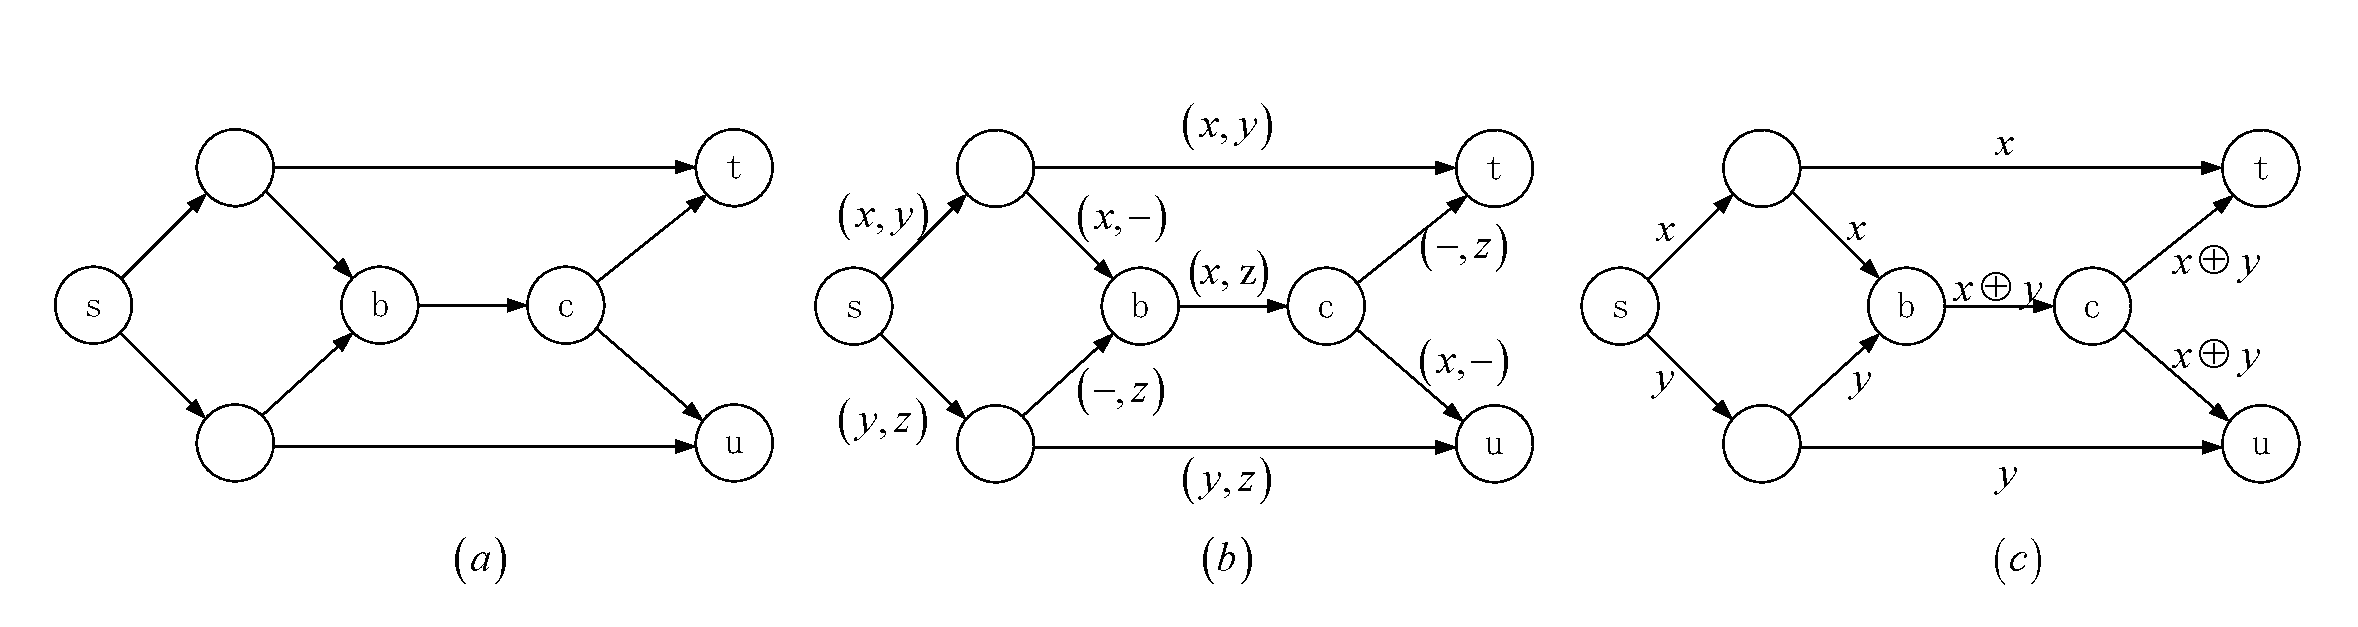
\includegraphics[width=6in]{figures/butter.eps}
	\caption{蝶形网络}
	\label{BUTTER_EPS}
\end{figure}
\par
图\ref{BUTTER_EPS}为一个包交换模型。在该网络中,源节点$s$需要将信息多播给两个目的的节点$t$和$u$。有向图的每一条有向边代表一条无差错包传输信道,每个 \emph{channel use}可以传输1个长为$m$比特的数据包。源节点希望以尽可能高的速率与两个目的节点通信。
\par
解决该问题,传统的路由方法如图\ref{BUTTER_EPS}$(b)$为例。在第一个时隙内,源节点$s$将$x$发送给$t$和$u$,将$y$发送给$u$。在第二个时隙内,源节点$s$将$y$传给了$t$,将$z$传给了$t$和$u$。两个时隙结束后,两个目的节点$t$和$u$都收到了$x$,$y$,$z$这三个数据包。可以看到,使用传统的路由方法,在两个时隙内可以传输3个不同的报文给$t$和$u$,因此传统路由方法的多播吞吐量为$\dfrac{3}{2} packet/channel\ use$。该多播吞吐量已被证明是使用路由方法能够实现的最大吞吐量。
\par
然而使用图\ref{BUTTER_EPS}$(c)$所示的网络编码方法,能够实现$2\ packet/per channel\ use$。该方法中,第一个时隙源节点$s$仍分发两个数据包$x$和$y$,与路由方法不同的是,节点$b$将对$x$和$y$进行异或运算,并转发运算结果。目的节点$t$收到数据包$x$和$x\oplus y$,并根据它们恢复出$x$和$y$。同样地,目的节点$u$也可以恢复出$x$和$y$。网络编码以网络中间节点的编码操作和目的节点的解码操作为代价,提升了网络的多播吞吐量,并突破了路由方法所能实现的吞吐量上限。是否有能比图\ref{BUTTER_EPS}$(c)$更好的方案?答案是没有。一个网络的最大多播吞吐量取决于分割源节点和目的节点的最小割集\textsuperscript{\cite{Ahlswede2000}}。图\ref{BUTTER_EPS}$(a)$的最小割集为2,故图\ref{BUTTER_EPS}$(c)$已经是最优方案。
\par
从上述例子中我们可以明白,要想充分利用通信网络的信息传输容量,光靠改进路由算法是不够的。在网络中,多个信息数据包可以通过多种方式有效地结合在一起,目的节点再从这些结合后的信息中恢复出原来数据包,达到提高网络的吞吐率的目的。
\subsection{网络编码的图论模型}
一个组合包网络$N=(V,E,S,T,A)$包括:
\begin{enumerate}[fullwidth,itemindent=2em,label=(\arabic*)]
	\item 有限有向无环多重图$G=(V,E)$,其中$V$表示图$G$的顶点集合,$E$表示图$G$的有向边的多重集合。
	\item 无重复源节点集合$S \subset V$,$S = \left\{ {{s_1},{s_2}, \cdots ,{s_{\left| S \right|}}} \right\}$。
	\item 无重复目的节点集合$T \subset V$,$T = \left\{ {{t_1},{t_2}, \cdots ,{t_{\left| T \right|}}} \right\}$。
	\item 有限的数据包集合$A$,$\left| A \right| \ge 2$。
\end{enumerate}
\par
图$G$的顶点代表包交换网络中的通信节点,有向边代表通信节点之间的无差错传输信道。有向边$(u,v)$具有单位容量,即每条边每次只能将一个数据包( 从符号集$A$中选取的一个符号)从$u$传送给点$v$。如果要进行更大容量的传输,可以在$u$和$v$之间建立多条平行边,单位容量都为1。以图\ref{TULUNMOXING_EPS}单源多宿网络为例,图\ref{TULUNMOXING_EPS}$\left(b\right)$与图\ref{TULUNMOXING_EPS}本质上是一样的,仅仅是将所有的路径都转换为单位容量。对于顶点$u,v \in V$,如果$v=u$或者图$G$中存在一条从$u$到$v$的有向路径,就称$u$可达$v$。在有向边$\left(u,v\right) \in E$上进行的操作是将点$u$发出的数据包$p \in A$无差错地交付给点$v$。
\begin{figure}[htbp]
	\centering
	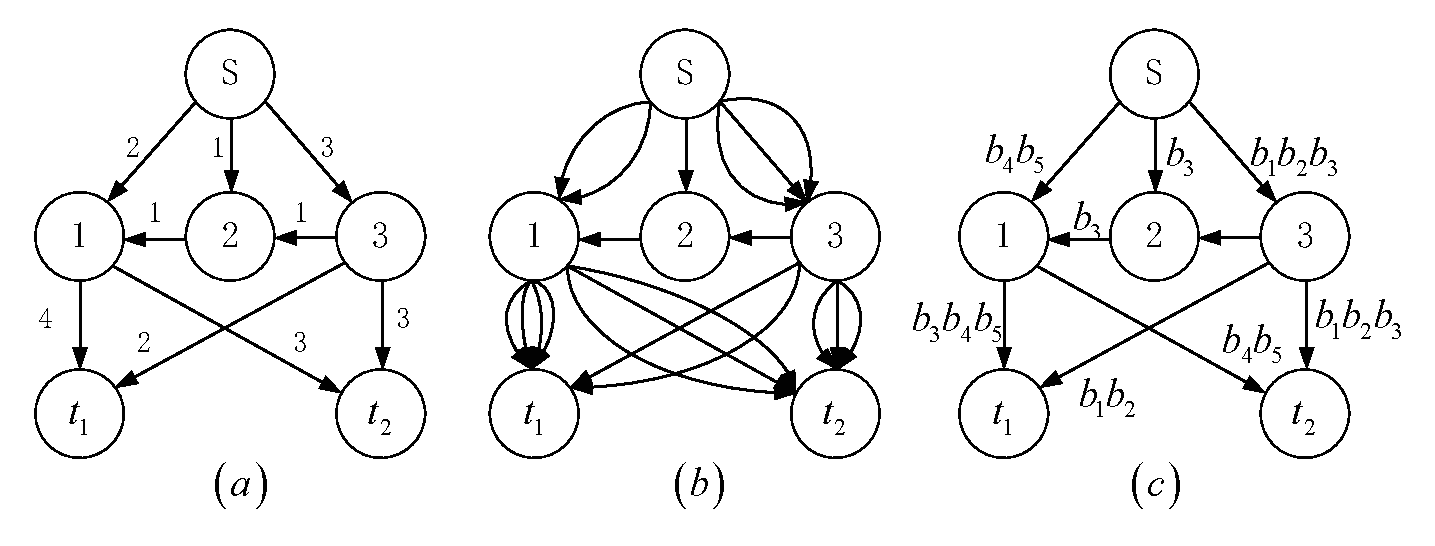
\includegraphics[width=6in]{figures/tulunmoxing.eps}
	\caption{单源多宿网络( 没有网络编码)}
	\label{TULUNMOXING_EPS}
\end{figure}
\par
对于顶点$v \in V$,我们用$I\left( v \right)$表示所有进入点$v$的边的集合,用$O\left( v \right)$表示所有从点$v$出发的边的集合。那么,组合包网络中的组合逻辑指的是:顶点$v$的出边集合$O\left( v \right)$中的任一非空闲边上传输的数据包是来自其入边集合$I\left( v \right)$中的所有非空闲数据包经过$v$的编码函数处理后得到的数据包集合。对于一个实际网络而言,在节点$v$通过某个数据包函数对入边集合的数据包进行处理,生成输出数据包之前,进入节点的数据包是需要被缓存的。
\par
节点$v$使用的函数被称为$v$的本地编码函数。当$v$只有路由功能时,它的出边上发送的数据包可以看做是对入边上收到的数据包的复制,即图\ref{TULUNMOXING_EPS}$\left( c \right)$所示的情况。图\ref{TULUNMOXING_EPS}$\left(c\right)$中,网络内部节点$1,2,3$仅仅通过存储转发的方法就达到了多播最大吞吐率,即源节点$s$可以同时发送5个数据包$b_{1}b_{2}b_{3}b_{4}b_{5}$给$t_{1}$和$t_{2}$。当$v$具有对入边数据包进行编码的功能后,如图\ref{BUTTER_EPS}$\left(c\right)$中节点$b$所示,网络多播吞吐率突破了仅仅使用路由方法的吞吐率上限。
\par
对于组合包网络,一次\emph{channel use}指的是为$E$中的每一条非空闲边都分配一个具体的数据包( 取自集合$A$ ),也可以看做是网路中的节点对特定编码函数的一次实现。换句话说,一次\emph{channel use}中的本地编码函数是固定的,且网络中的每条边最多被使用一次
\subsection{线性网络编码}\label{xianxingbianma}
我们用列向量$\left(p_{1},p_{2},\dots,p_{r}\right)^{T}$表示进入源节点$s$的数据包${{\rm X}_{{\rm I}\left( s \right)}}$。每个数据包$p_{i}$都是$\mathbb{F}_{q}$上的标量。对于更一般的多个数据包的情况,$p_{i}$可以看做是$\mathbb{F}_{q}$上长度为$m$的矢量。这样,我们可以用一个定义在$\mathbb{F}_{q}$上的$r \times m$矩阵来表示${\rm X}_{{\rm I}\left( s \right)}$,该矩阵的第$i$行是$p_{i}$。
\par
本地编码函数是$\mathbb{F}_{q}$上的线性函数,即任意中间节点$v$输出的数据包列向量${\rm X}_{{\rm O}\left( v \right)}$与其接收到的数据包列向量${\rm X}_{{\rm I}\left( v \right)}$之间的关系可以用以下线性方程组表示:
\begin{equation}\label{eq21}
{\rm X}_{{\rm O}\left( v \right)}={\rm L}_{v}{\rm X}_{{\rm I}_{\left( v \right)}}
\end{equation}
其中,${\rm L}_{v}$是定义在${\mathbb{F}}_{q}$上的系数矩阵,也称为节点$v$的本地转移矩阵。换句话说,$v$输出的每个数据包( ${\rm X}_{{\rm O}\left( v \right)}$的一个分量)都可以看做是进入$v$的多个数据包在$\mathbb{F}_{q}$上的线性组合。${\rm L}_{v}$的每一行都对应一条边$e \in {\rm O}\left(v\right)$,称为边$e$的本地编码向量。
\par
考虑到网络中只允许线性操作,因此任意边上传输的数据包都是原数据包$p_{1},p_{2},\dots,p_{r}$的线性组合。也就是$\forall v \in V$,有
\begin{equation}\label{eq22}
{\rm X}_{{\rm I}\left( v \right)}=G_{v}\left[ {\begin{array}{*{20}{c}}
	{{p_1}}\\
	\vdots \\
	{{p_r}}
	\end{array}} \right]
\end{equation}
其中,$G_{v}$是定义在$\mathbb{F}_{q}$上的系数矩阵,也称为$v$的全局转移矩阵。${\rm G}_{v}$的每一行都对应一条边$e \in {\rm I}_{\left( v \right)}$,称为边$e$的全局编码向量。
\par
图\ref{ZHUANYI_EPS}为标注了本地转移矩阵的蝶形网络。我们可以得到在目的节点$t$和$u$的全局转移矩阵为:
\begin{eqnarray}\label{eq23}
{G_t} = \left[ {\begin{array}{*{20}{c}}
	{{\alpha _1}{\alpha _5}}&{{\alpha _2}{\alpha _5}}\\
	{{\alpha _1}{\alpha _6}{\alpha _9}{\alpha _{11} }+{\alpha _3}{\alpha _7}{\alpha _{10}}{\alpha _{11} }}&{{\alpha _2}{\alpha _6}{\alpha _9}{\alpha _{11}}+{\alpha _4}{\alpha _7}{\alpha _{10}}{\alpha _{11}}}
	\end{array}} \right] \nonumber \\
{G_u}= \left[ {\begin{array}{*{20}{c}}
	{{\alpha _1}{\alpha _6}{\alpha _9}{\alpha _{12} }+{\alpha _3}{\alpha _7}{\alpha _{10}}{\alpha _{12} }}&{{\alpha _2}{\alpha _6}{\alpha _9}{\alpha _{12}}+{\alpha _4}{\alpha _7}{\alpha _{10}}{\alpha _{12}}}\\
	{{\alpha _3}{\alpha _8}}&{{\alpha _4}{\alpha _8}}
	\end{array}} \right]
\end{eqnarray}
\par
对于目的节点$t$来说,当且仅当$\left|{\rm I}\left(t\right)\right| \times r$阶全局转移矩阵$G_{t}$的秩为$r$时,$t$才能恢复出$\left(p_1,p_2,\dots,p_r\right)$中的所有元素。因为只有$G_t$满秩时,才存在满足${G_t}^{-1}G_t={\rm I}_r$的左逆矩阵,其中${\rm I}_r$是$r \times r$阶单位矩阵。只需$G_{t}$满秩,而不要求$G_{t}$是可求逆的方阵。目的节点$t$可以通过计算${G_t}^{-1}{\rm X}_{{\rm I}\left(t\right)}$得到$\left(p_1,p_2,\dots,p_r\right)^{T}$。
\begin{figure}[htbp]
	\centering
	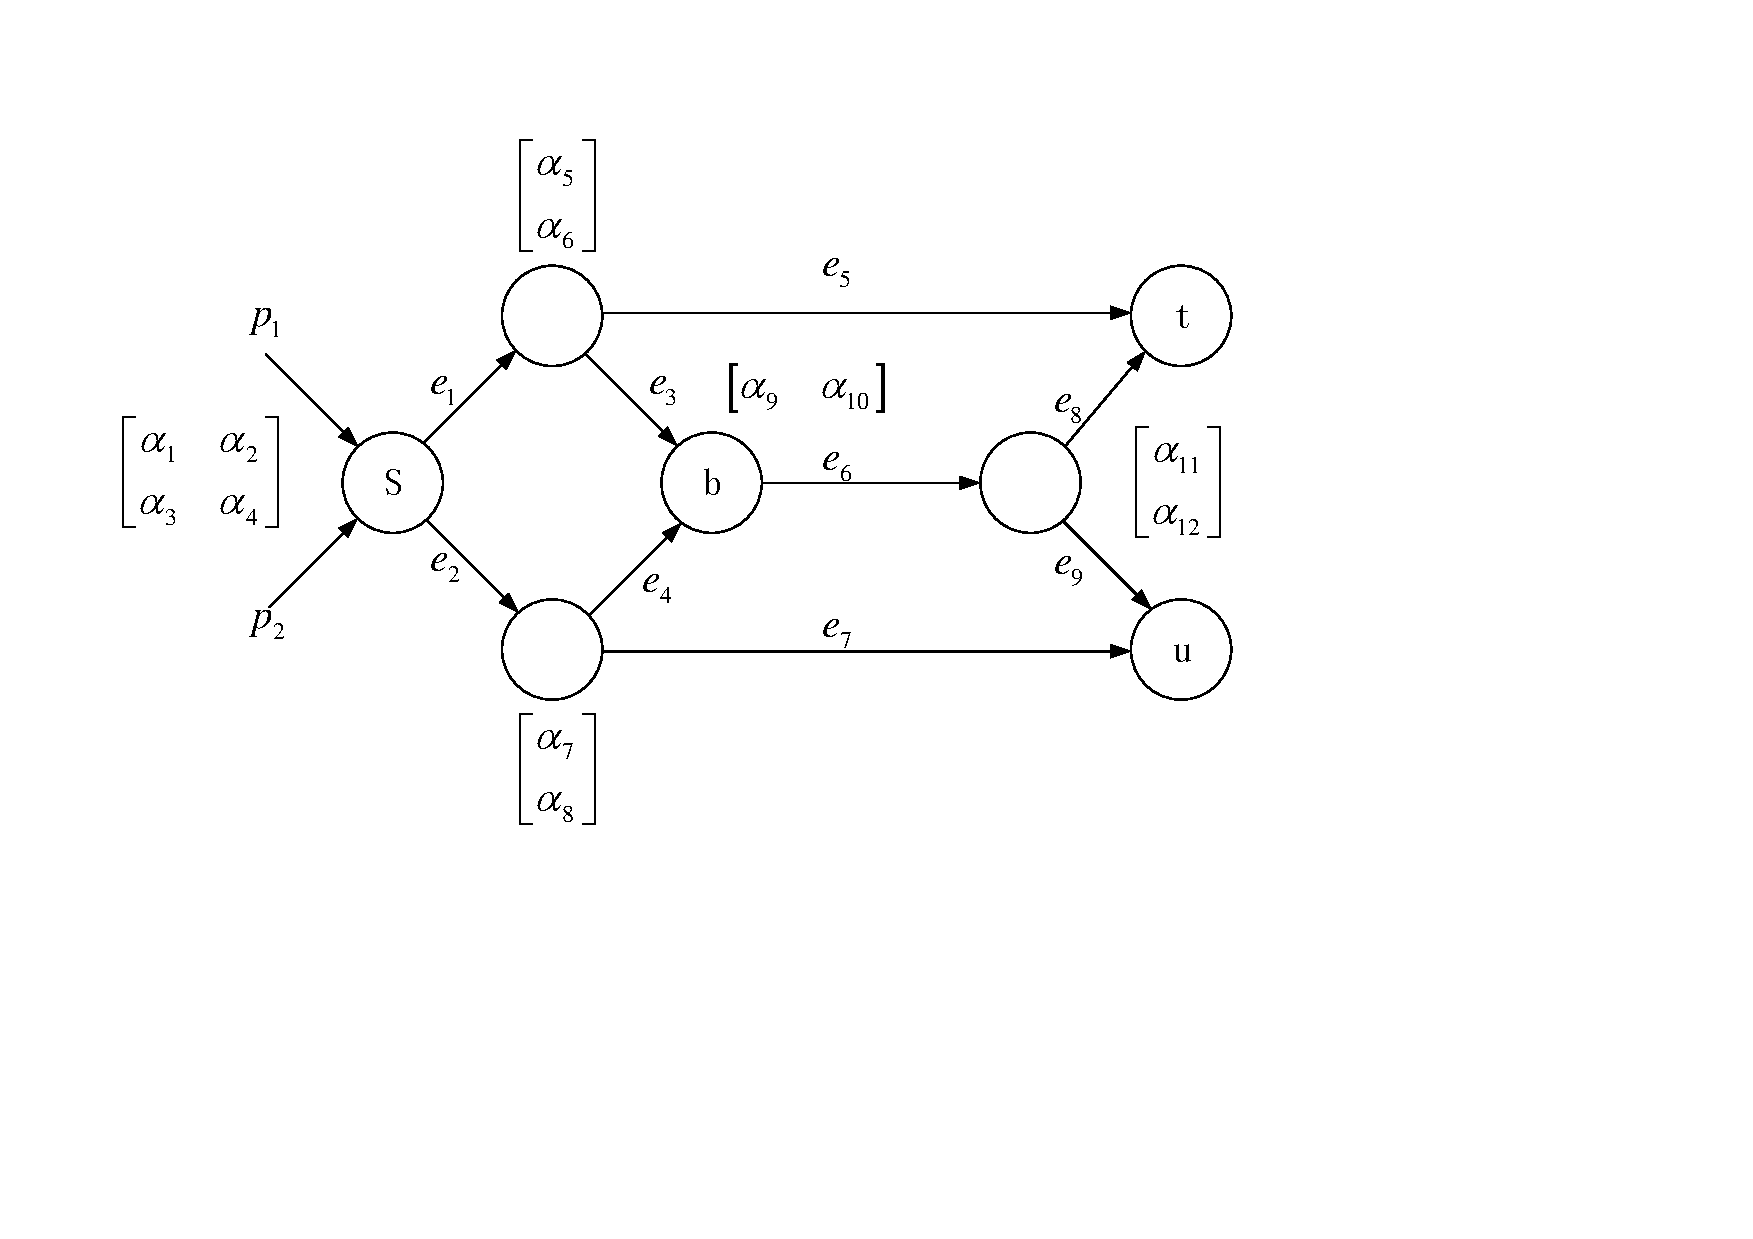
\includegraphics[width=4in]{figures/zhuanyi.pdf}
	\caption{标注了本地转移矩阵的蝶形网络}
	\label{ZHUANYI_EPS}
\end{figure}
\subsection{Network Coding 编码机制}
由于多径干扰、障碍物阻挡等原因,无线信道传输经常容易出错。链路层上比较著名的解决方法有前向纠错码( Forward Error Correction,FEC )和自动重传请求( Automatic Repeat Quest,ARQ )\textsuperscript{\cite{kurose2005computer}}。当错误是随机发生时,FEC可以有效地纠正报文的错误部分。FEC的优势是它不需要重传错误报文,也不会和TCP的原有机制产生冲突。FEC的缺点则是当链路质量很好地时候,会浪费带宽,而且会增加接收端CPU的计算和内存负担。同时,对于由于链路短暂断开导致的丢包,FEC也无能为力。当链路的丢包不是很频繁,还有传播时延不是很重要的时候,ARQ就比较有优势。然而,ARQ可能会与TCP的原有机制冲突\textsuperscript{\cite{kurose2005computer}}。为了有效控制丢包,有关学者将目光放在了基于FEC的编码机制上面,如纠删码( Erasure Coding )\textsuperscript{\cite{rizzo1997effective}}和网络编码\textsuperscript{\cite{Ahlswede2000,chou2003practical,algebraicapproach}}。
\par
网络中的数据包一般被看做是字节流。若干个数据包组成一个字节流,这个字节流被切分为$k$段,称为一个“\emph{generation}”\textsuperscript{\cite{chou2003practical}}。对于每一个\emph{generation},编码端使用随机线性编码产生$n$个经过编码的数据包。在目的节点,$n$个编码报文的任意$k$个独立数据包就足够恢复出原始数据包。换句话说,我们可以容忍网络中丢失$n-k$个报文。纠删码和网络编码的区别是前者只在源节点进行编码,而后者则在网络中的各个节点进行编码。实际上,纠删码可以看做是网络编码的特例。
\par
在恶劣的网络环境下,端到端的纠删码不足以实现可靠报文传输\textsuperscript{\cite{4753100}}。一些学者将网络编码应用于这些极具挑战性的网络中。和纠删码不同,网路的中间节点也会参与到编码中。在一些网络编码的实际应用中,“Batch Network Coding”是应用最为广泛的一种\textsuperscript{\cite{chachulski2007trading,algebraicapproach,chou2003practical,ho2003randomized,chen2009codecast,4015713}}。先介绍Batch Coding的相关原理。表\ref{SHUYU}是后面会用到的一些术语。
\begin{table}[htbp]
	\centering
	\caption{相关术语}
	\begin{tabularx}{350pt}{l|X}
		\toprule
		\textbf{名词} & \textbf{定义}\\
		\midrule
		Batch Coding & 每一个编码包会对同一个\emph{generation}里面的所有原始报文进行编码,只有\emph{generation}满秩之后才会进行编码或者解码\\
		\hline
		流水线编码 & 每当一个数据报文来之后,就会产生一个编码包,目的节点会逐步解出原始报文\\
		\hline
		\emph{generation} & 数据包的集合,作为编码和解码的整体\\
		\hline
		编码向量 & 反应组成某个编码数据包中各个原始数据包的系数\\
		\hline
		秩 & 线性独立的编码包的个数\\
		\hline
		编码冗余 & \emph{generation}的大小去除一个\emph{generation}生成的编码报文的个数得到的商\\
		\hline
		“Innovative”报文 & 一个可以增加秩的报文 \\
		\hline
		Delay & 目的站点的应用收到包的时间和包从源节点的应用产生的时间的差\\
		\bottomrule
	\end{tabularx}

\label{SHUYU}
\end{table}
\subsubsection[Batch Coding]{\textbf{Batch Coding}}
\par
假定在源节点有一个应用在不断产生同样大小的数据包\emph{$p_{1}$},\emph{$p_{2}$},\emph{$p_{3}$},$\dots$,。\emph{generation}的大小为$k$。第$i^{th}$个\emph{generation}产生的一个编码包可以被表示为:
\begin{equation}\label{eq24}
c = \sum\limits_{j = 1}^k {{e_j}{p_{i \times k + j}}}
\end{equation}
这里$e_{k}$是某个有限域$\mathbb{F}$中的一个元素,$i \times k$是在第$i$个\emph{generation}之前传输的的包的个数。每个数据包都被看做是在有限域$\mathbb{F}$上的一个向量,所有操作都是在有限域$\mathbb{F}$上进行。令$r$表示编码冗余度,$r  \ge 1$。对于每一个\emph{generation},源节点会产生$k \times r$个编码包。在目的节点,收到$k$个线性独立的包后,目的节点通过高斯消元解公式\ref{eq25},就可以恢复出原来$k$个数据包。
\begin{equation}\label{eq25}
\left[ {\begin{array}{*{20}{c}}
	{{c_1}}\\
	\vdots \\
	{{c_k}}
	\end{array}} \right] = \left[ {\begin{array}{*{20}{c}}
	{e_1^{\left( 1 \right)}}& \cdots &{e_k^{\left( 1 \right)}}\\
	\vdots & \ddots & \vdots \\
	{e_1^{\left( k \right)}}& \cdots &{e_k^{\left( k \right)}}
	\end{array}} \right]\left[ {\begin{array}{*{20}{c}}
	{{p_1}}\\
	\vdots \\
	{{p_k}}
	\end{array}} \right]
\end{equation}
\par
由于每个编码数据包都是同一个\emph{generation}的数据包的线性组合,在源节点就引入了一个延时。换句话说,同一个\emph{generation}里面前面的报文需要等后面的报文,直到这个\emph{generation}满秩后,才可进行编码。在目的节点处,同一个\emph{generation}的报文,要么都解码,要么一个都解不出。
\par
为了刻画Batch Coding整个的时延,我们定义“delay”如下:接收端的应用收到报文的时间和源节点的应用产生报文的时间的差值。$t_{i}$表示源节点产生{\textbf{data}}\textsubscript{\textbf{i}}的时间,$t_{ci}$表示第$i$个编码包被发出去的时间。假定报文传输过程中的处理时延、传输时延、传播时延和排队时延都是常数,$d_{n}$表示网络中出现的时延的总和,$d_{c}$表示接收端的解码过程的时延,也为一个常数。假定一个\emph{generation}还有$k$个数据包,那么在无损信道中,传送数据包{\textbf{data}}\textsubscript{\textbf{i}}的时延为:
\begin{equation}\label{eq26}
{t_{c\left\lceil {{i \mathord{\left/
					{\vphantom {i k}} \right.
					\kern-\nulldelimiterspace} k}} \right\rceil *k}} - {t_i} + {d_n} + {d_c}
\end{equation}
\begin{figure}[htbp]
	\centering
	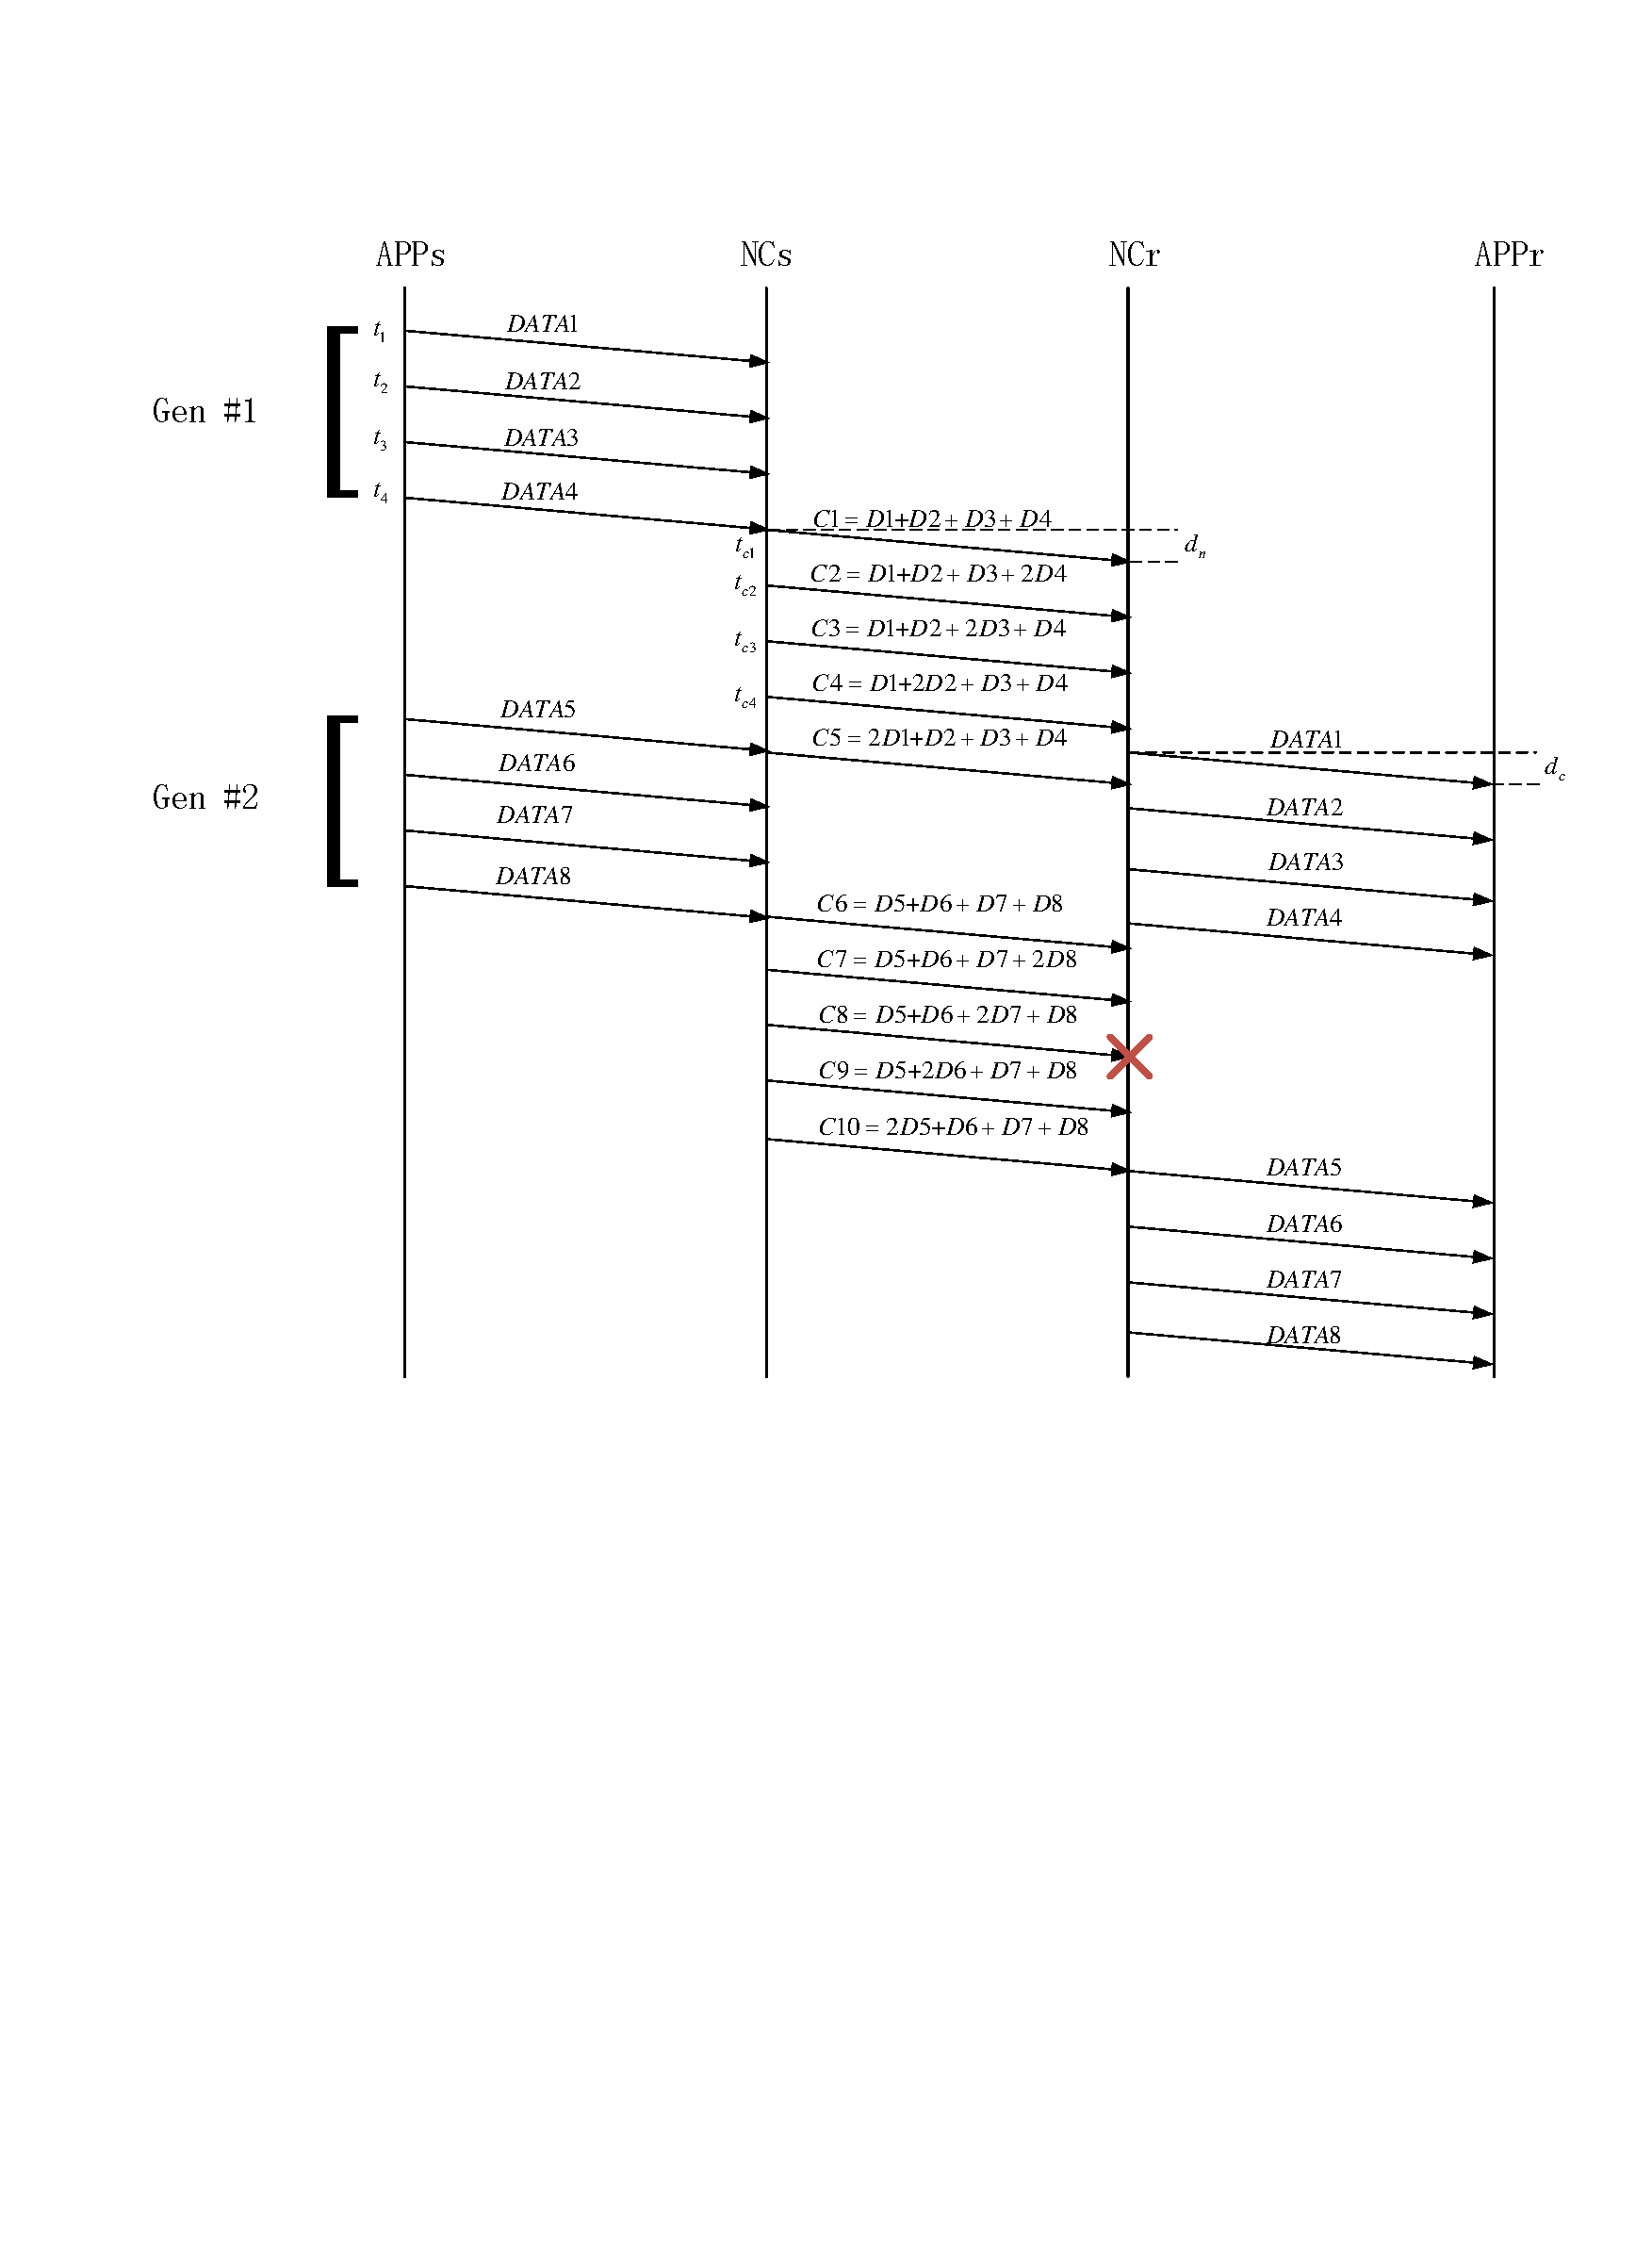
\includegraphics[width=6in]{figures/batch.pdf}
	\caption{Batch Coding 例子}
	\label{BATCHCODING_EPS}
\end{figure}
例如,在图\ref{BATCHCODING_EPS}中,传送\emph{data\textsubscript{1}}的时延为$t_{c4}-t_{1}+d_{n}+d_{c}$。这里\emph{generation}的大小为4,编码冗余为1.25.因此对于每个\emph{generation}来说,都会发送$k*r=5$个编码包。
\par
如果链路中出现丢包,接收端只需要收到4个线性独立的编码包就可以解出对应的\emph{generation}的所有原始数据报文。图\ref{BATCHCODING_EPS}中的“generation \# 2”描述了一个丢包被恢复,解码端成功解码的例子。然而如果冗余度不够补偿丢失的话,那么这个\emph{generation}就没有报文被解出来。如图\ref{BATCHUNDECODE_EPS},丢了$C4$和$C5$,接收端无法解码。
\begin{figure}[htbp]
\centering
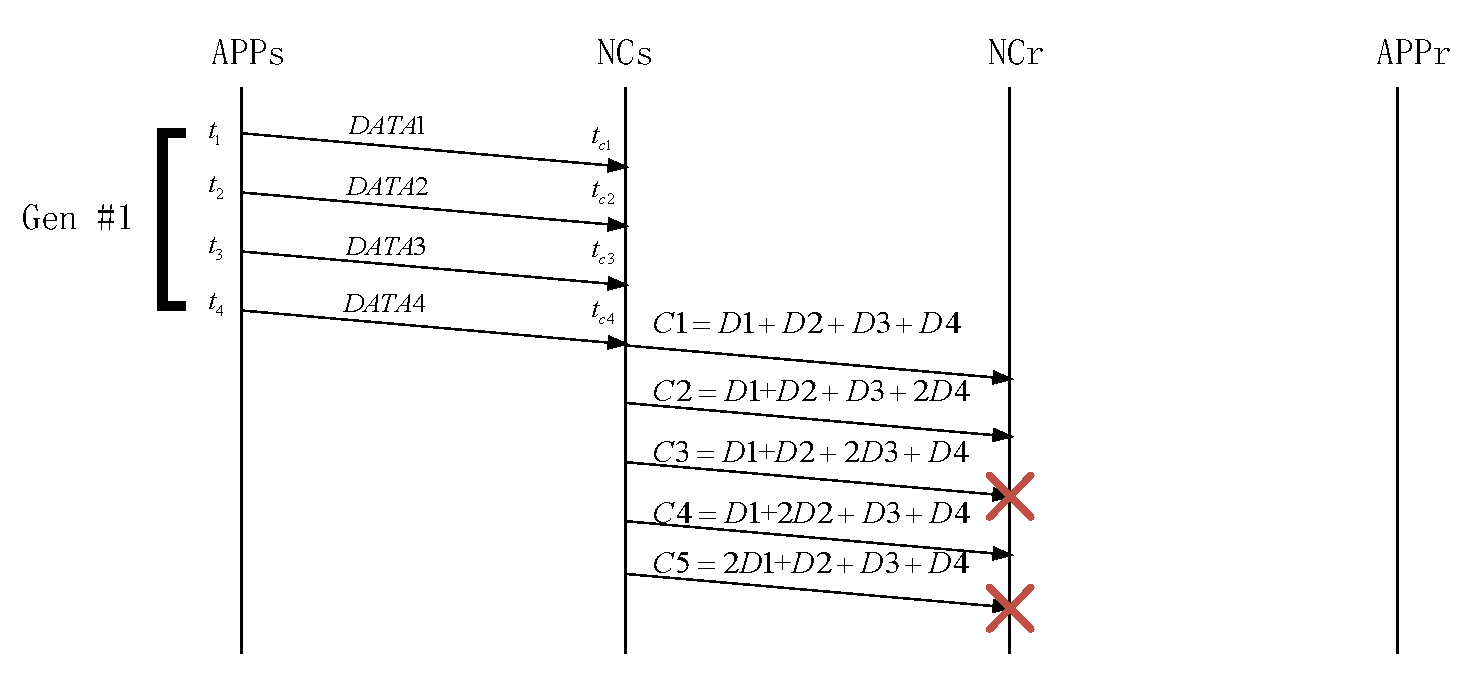
\includegraphics[width=6in]{figures/batchundecode.eps}
\caption{Batch Coding 例子:不可解}
\label{BATCHUNDECODE_EPS}
\end{figure}
\par
“Batch Network Coding”指的是这样一类编码:源节点和网络中的中间节点在同一个\emph{generation}上进行编码,目的节点只有在收到足够多的编码报文后,才能一次性解出这一个“\emph{generation}”中的所有原始报文。 
\par
Batch Network Coding有两个显著的缺点:首先,它引进了和\emph{generation}大小成比例的编解码时延,对于实时性要求比较高的应用来说,会限制\emph{generation}的大小,也就会降低编码的弹性;其次,只有当接收到足够多的线性独立的编码报文后,才可以解出一个\emph{generation}的所有报文,否则,整个\emph{generation}会被丢弃。
\par
文献\cite{chen2010pipeline}的作者针对Batch Network Coding的弱点提出了流水线网络编码( Pipeline  Network Coding )。
\subsubsection[Pipeline Coding]{\textbf{流水线编码}}\label{pipelinesec}
流水线编码旨在减少编解码时延,进而提高吞吐率。和Batch Coding不一样的是,流水线编码不需要等集满一个\emph{generation}大小的报文后才进行编码,与公式\ref{eq24}稍微不同,流水线编码的编码函数为:
\begin{equation}
c = \sum\limits_{j = 1}^m {{e_j}{p_{i \times k + j}}}
\end{equation}
其中,$m$为目前在编码缓存中的数据包个数。换句话说,如果收到一个原始报文,发送端基于目前收到的数据包立马执行一个编码函数。如果所有的编码包都依次正确地送到目的节点,那么目的节点可以构建如下的下三角矩阵:
\begin{equation}\label{eq28}
\left[ {\begin{array}{*{20}{c}}
	{{c_1}}\\
	\vdots \\
	{{c_k}}
	\end{array}} \right] = \left[ {\begin{array}{*{20}{c}}
	{e_1^{\left( 1 \right)}}&0& \cdots &0\\
	{e_1^{\left( 2 \right)}}&{e_2^{\left( 2 \right)}}&{}& \vdots \\
	\vdots &{}& \ddots &0\\
	{e_1^{\left( k \right)}}&{e_2^{\left( 2 \right)}}& \cdots &{e_k^{\left( k \right)}}
	\end{array}} \right]\left[ {\begin{array}{*{20}{c}}
	{{p_1}}\\
	\vdots \\
	{{p_k}}
	\end{array}} \right]
\end{equation}
上述方程可以逐步求解,而无需等待整个的\emph{generation}报文都集齐。例如,收到$c_{1}$,目的节点可以解码出$p_{1}$,以此类推。编码冗余的设计与Batch Coding略有不同。令$r$为编码冗余度,$r \ge 1$。对于每个数据包来说,$r - \left\lfloor r \right\rfloor $的概率产生$\left\lfloor r \right\rfloor + 1$个编码包,$1 - \left({r - \left\lfloor r \right\rfloor} \right)$的概率产生$r$个编码包。
\begin{figure}[htbp]
	\centering
	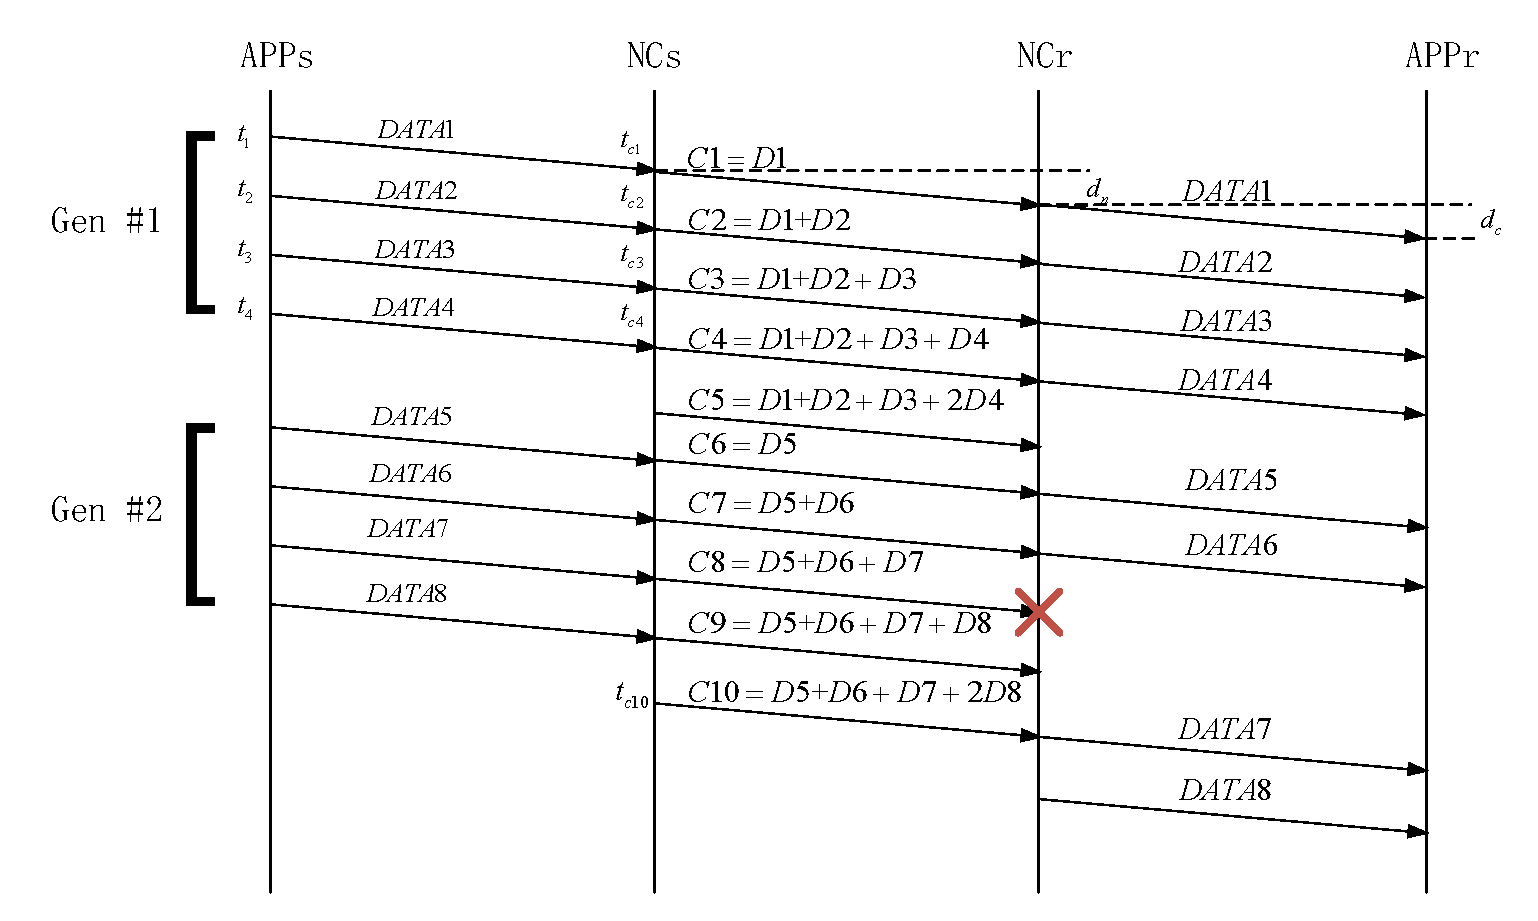
\includegraphics[width=6in]{figures/pipeline.eps}
	\caption{流水线编码}
	\label{LIUSHUIXIAN_EPS}
\end{figure}
\par
与前面分析Batch Coding时一样,我们让$t_{i}$表示源节点产生数据\textbf{data}\textbf{\textsubscript{i}}的时间,$t_{ci}$表示第$i$个编码数据包被发出去的时间。那么传送数据包\textbf{data}\textbf{\textsubscript{i}}的时延为$t_{ci} - t_{i}+d_{n}+d_{c}$。在大多数情况下,这比公式\ref{eq26}所表示的时延小多了。
\par
图\ref{LIUSHUIXIAN_EPS}展示了一个流水线编码的例子。这里\emph{generation}的大小为4,冗余度为1.25。当有一个原始数据包产生时,立马就编码得到一个编码包。同样地,在解码端,每当有一个“innovative”报文到来的时候,就可以立马解出一个原始报文。
\par
对于丢包的情况,图\ref{LIUSHUIXIAN_EPS}中\emph{Gen \# 2}中的$C8$丢失,目的节点在收到$C9$后,无法解出$DATA7$。这时候需要将undecoded packets存起来,等到冗余报文过来才可以解出原始报文,如图\ref{LIUSHUIXIAN_EPS}中的$C10$。Batch Coding的编解码流程如Algorithm\ref{algo1}和Algorithm\ref{algo2}。
\par
采用流水线编码的优点主要有:
\begin{enumerate}[fullwidth,itemindent=2em,label=(\arabic*)]
	\item 更低的解码时延
	\item 更高的吞吐率
	\item 对上层来说是透明的( UDP,TCP,或者其他协议 )
\end{enumerate}
\par
本文所实现的TCP/NC协议也是基于流水线网络编码。
\begin{algorithm}
	\caption{Encoding Function}  
	\label{algo1}
	\KwIn{coding redundancy $r$,data packet \emph{data} from up-layer,$generation\_buffer\left[0,\dots,m,\dots \right]$,number of packets currently in \emph{generation buffer} $m-1$}  
	\KwOut{NONE}  
	Store $data$ to \emph{generation buffer}\;
	%%$i$ \leftarrow $0$ \;
	$i \leftarrow 0$\;
	\While{$i<num$}  
	{  
		\If{$\left(num-i<1 \wedge rand()\% 100 > num-i\right)$}  
		{  
			\Break\;
		} 
		Generate Coding Vector\;
		\For{$j=0;j \le m-1;j++$}
		{
			\If{$generation\_buffer[j]==NULL$}{$coding\_vector[j]=0$}
		}
		Encode packet\;
		Send Coded Packet to MAC layer\;
		%%$i$ \leftarrow $i+1$\;
		$i \leftarrow i+1$\;
	}
\end{algorithm}
	\begin{algorithm}
		\caption{Decoding Function}
		\KwIn{data packet \emph{data},$generation\_buffer\left[0,\dots,m,\dots \right]$}
		\KwOut{NONE}
		\label{algo2}  
		\If{(\emph{not\_innovative}(data))}
		{
			Free\_data(\emph{data})\;
			\Return;
		}
		Store \emph{data} to \emph{generation buffer}\;
		Gaussian\_Elimination(\emph{generation})\;
		\If{(decodable packets cause no reordering)}
		{
			Deliver it to Transport Layer;
		}
	\end{algorithm}


\section{TCP/NC协议}
在详细阐述TCP/NC协议原理之前,先引入\emph{ACK on degree of freedom}这个概念。
\par
\subsection{ACK on degree of freedom}\label{ackondegree}
现有的很多可靠传输协议都有ACK这个机制,如TCP,ARQ等。接收方通过回复发送方ACK来让发送方了解自己收到了哪些数据。如果在没有应用编码的网络中,那么接收端在收到原始报文后就可以回给发送方ACK;如果在应用了网络编码的网络中,如文献\cite{Lun2008On},接收端需要在收到若干个数据包后,对整体进行解码恢复原始数据包,才会回复ACK,亦如第二章介绍的Batch Coding,其缺点是传送数据包的时延较长。针对Batch Coding的缺点,文献\cite{chen2010pipeline}提出了流水线编码( Pipeline  Coding ),但是在丢包网络中也会存在ACK延迟的问题。图\ref{LIUSHUIXIAN_EPS}中的$DATA7$和$DATA8$需要等到收到$C10$后才可以解出,进而回给发送端ACK。ACK的延迟不仅会影响吞吐率,还会影响发送端的编码队列的长度。直觉来说,编码端只有在收到某个数据包的ACK后,才会将其从编码缓存中删除。例如,源节点有$n$个数据包( 每个数据包看做是有限域$\mathbb{F}$上的向量 ),分别是$p_{1}$,$p_{2}$,$\dots$,$p_{n}$。经过编码,依次发出去$n$个编码包,分别是$p_{1}$,$\left(p_{1}+p_{2}\right)$,$\left(p_{2}+p_{3}\right)$,$\dots$,$\left(p_{n-1}+p_{n}\right)$。由于网路质量差,第一个包$p_{1}$丢了,接收端只收到$\left(p_{1}+p_{2}\right)$,$\left(p_{2}+p_{3}\right)$,$\dots$,$\left(p_{n-1}+p_{n}\right)$。接收端尽管收到了$n-1$个编码包,但一个也无法解出来,也就无法给源节点确认ACK。可靠传输要求发送端在没收到接收端确认ACK时必须把$p_{1}$,$p_{2}$,$\dots$,$p_{n}$都放入缓存队列。我们可以看到这个队列此时的长度长达$n$。
\par
针对以上问题,文献\cite{4595268}首次提出了“ACK on degree of freedom”的概念。在介绍“ACK on degree of freedom”之前,我们先引入一个定义。
\begin{myDef}[Seeing a packet]\label{df26}
	如果一个节点根据现有的信息可以计算出如\textbf{\emph{$\left(p+q\right)$}}形式的线性组合,那么我们就说这个节点“\textbf{see packet \emph{$p$}}”。其中\textbf{$q$}本身就是只包含序号比$p$大的报文的线性组合。解码出某个报文也算作是“seeing a packet”,此时\textbf{$q=0$}。

\end{myDef}
\par
直觉告诉我们,如果目的节点已经\emph{see packet $p$},那么发送端那边在产生编码包的时候,就不必将数据包$p$再囊括进去了。换句话说,发送端可以将数据包$p$从编码缓存中移除。接收端如果后面接收到足够的信息,将$q$解出来,那么$p$自然就解出来了。因此,接收端如果已经\emph{see packet $p$},那么其可以直接向发送端回复ACK,表示自己已经收到了报文$p$,通知发送端那边将报文$p$从编码缓存中移除。
\par
表\ref{tab:drop-when-seen}展示的就是\emph{ACK on degree of freedom} 的一个例子。在时隙1时,发送端发送了报文$p_{1}$,$p_{1}$在链路中丢失了,目的节点\emph{A}没有收到;在时隙2时,由于\emph{A}没有发送对报文$p_{1}$的ACK,所以源节点发送缓存为$p_{1}$和$p_{2}$,接着发送端对$p_{1}$和$p_{2}$进行异或,得到编码包,发出去。目的节点收到了编码包,虽然无法解出$p_{1}$和$p_{2}$,但根据定义\ref{df26},\emph{A}看到了$p_{1}$。因此,\emph{A}回复源节点一个ACK,让源节点将$p_{1}$从编码缓存中移除。我们可以看到,在时隙3时,源节点的发送缓存只有$p_{2}$和$p_{3}$,和前面一样,源节点发送编码包$p_{2} \oplus p_{3}$。这一次\emph{A}正确地收到了,\emph{A}看到了$p_{1}$和$p_{2}$,但还是无法解出它们。我们看到,一直到时隙5,\emph{A}都没有解出一个报文,但看到的报文( seen packet )有$p_{1}$,$p_{2}$,$p_{3}$。源节点在时隙6发送了$p_{4}$,导致$p_{5}$被看到,然后在时隙7发送了$p_{5}$,让\emph{A}解出了所有报文。
\begin{table}[htbp]  
	\centering  
	\fontsize{6.5}{8}\selectfont  
	\begin{threeparttable}  
		\caption{\emph{ACK on degree of freedom} 例子}  
		\label{tab:drop-when-seen}  
		\begin{tabular}{c|c|c|c|c|c}  
			\toprule  
			\multirow{2}{*}{Time} &\multirow{2}{*}{Sender's queue} & \multirow{2}{*}{Transmitted packet} & \multirow{2}{*}{Channel state}&  
			\multicolumn{2}{c}{ Destination Node \emph{A}}\cr  
			\cmidrule(lr){5-6}  
			\hspace{1cm}&\hspace{1cm}&\hspace{1cm}&\hspace{1cm}&Decoded&Seen but not decoded\cr  
			\midrule  
			1&$p_{1}$&$p_{1}$&$\nrightarrow A$&\hspace{1cm}&\hspace{1cm}\cr
			\hline  
			2&$p_{1}$,$p_{2}$&$p_{1} \oplus p_{2}$&$\rightarrow A$&\hspace{1cm}&$p_{1}$\cr 
			\hline 
			3&$p_{2}$,$p_{3}$&$p_{2} \oplus p_{3}$&$\rightarrow A$&\hspace{1cm}&$p_{1}$,$p_{2}$\cr
			\hline  
			4&$p_{3}$,$p_{4}$&$p_{3} \oplus p_{4}$&$\nrightarrow A$&\hspace{1cm}&$p_{1}$,$p_{2}$\cr
			\hline  
			5&$p_{3}$,$p_{4}$,$p_{5}$&$p_{3} \oplus p_{4} \oplus p_{5}$&$\rightarrow A$&\hspace{1cm}&$p_{1}$,$p_{2}$,$p_{3}$\cr
			\hline  
			6&$p_{4}$&$p_{4}$&$\rightarrow A$&$p_{4}$&$p_{1}$,$p_{2}$,$p_{3}$,$p_{5}$\cr
			\hline
			7&$p_{5}$&$p_{5}$&$\rightarrow A$&$p_{1}$,$p_{2}$,$p_{3}$,$p_{4}$,$p_{5}$&\hspace{1cm}\cr    
			\bottomrule  
		\end{tabular}  
	\end{threeparttable}  
\end{table}  
\par
总结一下,\emph{ACK on degree of freedom}就是说我不再对原始数据包进行ACK确认,而是确认\emph{自由度}。只要接收端看到了某个报文( see a packet ),即使没有解出来,依然可以回复发送端对seen packet的确认。
\subsection{TCP/NC原理}
\par
网络编码自出现以来就作为一种重要的改善网络性能,尤其是无线网络性能的工具。它的主要优势在于能够跨时间、跨流地将数据混合起来。这可以让在lossy信道中的数据传输更为健壮和高效。尽管如此,我们还是很少看见应用网络编码的实际例子,一个主要原因就是如何将网络编码很自然地加入到现有的网络体系中,而不与其冲突。
%文献\cite{4298308}阐述了反馈如何应用到网络编码中,具体到TCP来说,就是如何利用原有的ACK机制作为我们的网络编码的反馈。
\par
Sundararajan等人在“Network Coding Meets TCP”\textsuperscript{\cite{Sundararajan2009}}一文中提出编码TCP协议( TCP/NC),用于提高标准TCP协议在无线网络环境下的性能。其通过在TCP层和IP层之间添加一个网络编码层来掩盖lossy信道中出现的随机丢包。与以往一些学者在改进TCP在无线网络下性能的工作不同的是,TCP/NC不需要对原有的OSI协议栈做出修改。TCP/NC可以很优雅地与标准TCP协议,IP协议,链路层的协议一起工作,不会与原有协议的机制冲突,适合大规模地部署在现有互联网体系中。
\par
TCP可靠传输的背后思想是使用Acknowledgements对按序到来的数据包进行确认,同时发送端使用ACK来进行拥塞控制。对于使用网络编码来说,这个机制需要做点改变。其原因在于使用网络编码后,接收端收到的不再是原始数据包,而是原始数据包的线性组合( 这里仅针对线性网络编码 )。一旦收到足够多的线性组合,就可以解码得到原始数据包。标准TCP中“\emph{按序到达的报文}”这个概念缺失了。现有的ACK机制不允许我们确认还未解码的数据包。上一小节所讲到的\emph{ACK on degree of freedom}概念值得借鉴。绝大多数情况,接收端收到的线性组合报文都会给接收端带来新信息( 在有限域$\mathbb{F}$下有可能出现非线性独立的编码包 ),也就是自由度( 将编码数据包看做是向量 )。TCP/NC对于收到的编码包产生的自由度回复ACK,表示自己看到了某个包$p$\footnote{seen packet的概念见\ref{ackondegree}小节的定义\ref{df26}},而不管这个新来的包是否让接收端解出了一个包。
\par
图\ref{TCPNC_EPS}为TCP/NC的系统框架。在TCP层和IP层之间引入了一个NC编码层。NC层缓存从TCP层下来的数据包,并放入编码缓存,然后生成处于编码缓存中所有数据包的线性组合并发出去。当发送端的NC层收到接收端的ACK后,才会将对应的数据包从编码缓存中删除,并将相应ACK传给上层TCP。编码包在到达接收端的NC层之后会被放入解码缓存,并进行高斯消元等解码操作。如若有新的包被看到,则回复发送端相应的ACK;如若有数据包被解出,将其交给上层TCP。
\begin{figure}[htbp]
	\centering
	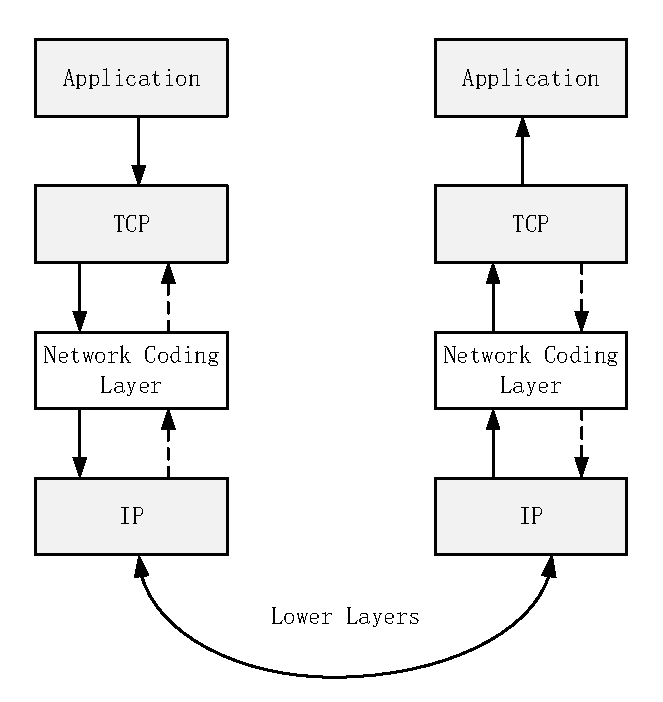
\includegraphics[width=3in]{figures/tcpnc.eps}
	\caption{TCP/NC协议架构}
	\label{TCPNC_EPS}
\end{figure}
\par
TCP/NC能够抵抗链路丢包的关键就是发送端进行冗余编码。通过“seen”这个概念,将链路丢包这个问题往后推。如果后期的冗余包能够补偿丢失的报文,那么TCP层就不会发现丢包。如图\ref{CODINGACK_EPS}所示,虽然$SEQ=2$和$SEQ=3$这两个报文丢失,但发送端依然可以收到对$p_{2}$和$p_{3}$的ACK。只要后期传输过程中的冗余包足够补偿掉$SEQ=2$和$SEQ=3$的丢失,那么上层TCP就根本发现不了丢包。理论上,当链路的丢包率为$\rho$时,设置的冗余度应该为$R=\frac{1}{1-\rho}$。
\begin{figure}[htbp]
	\centering
	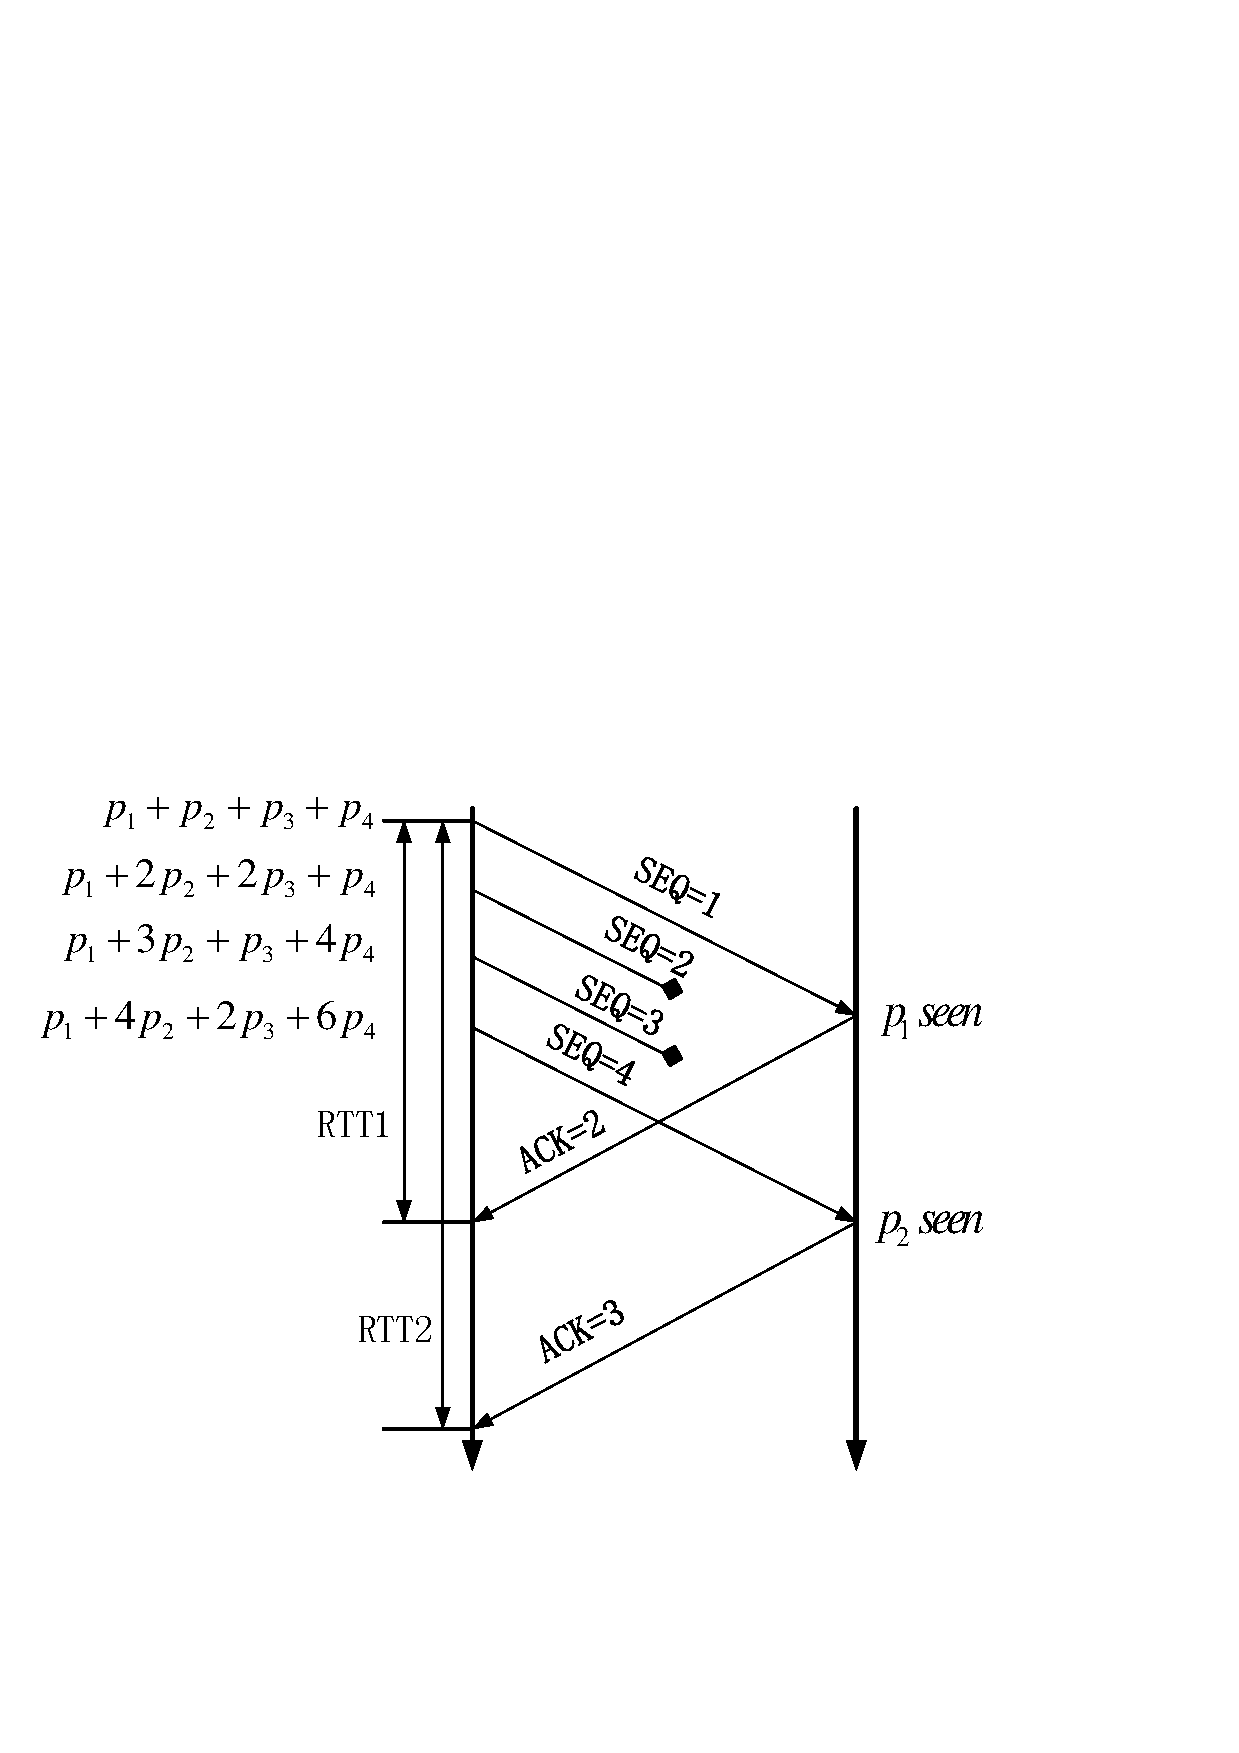
\includegraphics[width=4in]{figures/codingack.pdf}
	\caption{编码和ACK示例}
	\label{CODINGACK_EPS}
\end{figure}
\section{本章小结}
本章首先介绍了网络编码的相关理论,对其图论模型做了描述,并在此基础上阐述了线性网络编码的相关知识。然后介绍了目前在网络编码领域应用最为广泛的Batch Coding编码机制,分析了其优缺点,引出了流水线编码机制,给出了编解码算法。最后介绍了TCP/NC协议的原理架构,重点提及了其引入的几个新概念,如“seen packet”,分析其是如何抵抗网络丢包的。本章主要是为后面的TCP/NC协议的实现和改进打下基础。 

%---------------------------------------------------------------------------------
%                西南交通大学研究生学位论文:第三章内容
%---------------------------------------------------------------------------------
\chapter{TCP/NC协议实现}
本章主要讲TCP/NC的具体实现,在无线lossy信道下测试TCP/NC的性能,并与标准的TCP-vegas进行分析对比。
\section{数据包编码}
在阐述数据包编码之前,先简单介绍近世代数的相关概念。
\subsection{有限域与扩域}
\begin{myDef}[阿贝尔群]
	对于一个非空元素集合$G$以及定义在$G$上的一种运算“$*$”( 这里的$*$泛指一种代数运算,如$+$,$-$,$\times$,$\div$,模$m$加$\oplus$,模$m$乘$\odot$等)。若满足以下四个条件:
	\begin{enumerate}[fullwidth,itemindent=2em,label=(\arabic*)]
		\item 封闭性,即$\forall a,b \in G$,$\exists\left(a*b\right)=c\in G$。
		\item 结合性,即$\forall a,b \in G$,$\exists a*\left(b*c\right)=\left(a*b\right)*c$。
		\item 存在唯一一个单位元$e$,即$\forall a \in G$,$\exists a*e=e*a=a$。
		\item $G$中的每个元素各自存在唯一的逆元,即$\forall a \in G$,$\exists {a^{ - 1}} \in G$,使得$a*{a^{-1}}={a^{-1}}*a=e$。这里${a^{-1}}$泛指逆元。
		\item $\forall a,b \in G$,$\exists a*b=b*a$
	\end{enumerate}
	\par
	则称这样的代数系统为阿贝尔群,记做$\left(G,*\right)$\textsuperscript{\cite{zzc2003}}。
\end{myDef}
\begin{myDef}[有限域]
	非空集合$F$含有有限个元素,其中定义了加和乘两种运算,且满足
	\begin{enumerate}[fullwidth,itemindent=2em,label=(\arabic*)]
		\item $F$关于加法构成阿贝尔群,加法恒等元记为0
		\item $F$中所有非零元素对乘法构成阿贝尔群,乘法恒等元记为1
		\item $F$加法和乘法满足分配律
	\end{enumerate}
	\par
	则$F$与这两种运算构成有限域\textsuperscript{\cite{zzc2003}}。
\end{myDef}
\begin{table}[htbp]
	\centering
	\caption{本原多项式$P\left(x\right)=x^{4}+x+1$的根生成的循环群}
	\begin{tabularx}{250pt}{c|c|c}
		\toprule
		\textbf{各次幂$\alpha_{k}$} & \textbf{$\alpha$的多项式}&\textbf{多项式系数$m$重}\\
		\midrule
		$\alpha^{0}$ & 1 &$\left(0001\right)$\\
		\hline
		$\alpha^{1}$ & $\alpha$ &$\left(0010\right)$\\
		\hline
		$\alpha^{2}$ & $\alpha^{2}$ & $\left(0100\right)$\\
		\hline
		$\alpha^{3}$ & $\alpha^{3}$ & $\left(1000\right)$\\
		\hline
		$\alpha^{4}$ & $\alpha+1$ & $\left(0011\right)$\\
		\hline
		$\alpha^{5}$ & $\alpha^{2}+\alpha$ & $\left(0110\right)$\\
		\hline
		$\alpha^{6}$ & $\alpha^{3}+\alpha^{2}$ & $\left(1100\right)$\\
		\hline
		$\alpha^{7}$ & $\alpha^{3}+\alpha+1$ & $\left(1011\right)$\\
		\hline
		$\alpha^{8}$ & $\alpha^{2}+1$ & $\left(0101\right)$\\
		\hline
		$\alpha^{9}$ & $\alpha^{3}+\alpha$ & $\left(1010\right)$\\
		\hline
		$\alpha^{10}$ & $\alpha^{2}+\alpha+1$ & $\left(0111\right)$\\
		\hline
		$\alpha^{11}$ & $\alpha^{3}+\alpha^{2}+\alpha$ & $\left(1110\right)$\\
		\hline
		$\alpha^{12}$ & $\alpha^{3}+\alpha^{2}+\alpha+1$ & $\left(1111\right)$\\
		\hline
		$\alpha^{13}$ & $\alpha^{3}+\alpha^{2}+1$ & $\left(1101\right)$\\
		\hline
		$\alpha^{14}$ & $\alpha^{3}+1$ & $\left(1001\right)$\\
		\hline
	\end{tabularx}
	\label{SHUYU}
\end{table}
\par
有限域提供了一个有限集,在该有限集上明确地定义且有效地实现了加法、减法、乘法及除法运算( 减法可以转换为加法,除法可以转换为乘法),并允许系统使用矩阵、行列式、高斯消元等线性代数中常见的运算工具来解决该域上的联立线性方程组问题。
\par
我们在讲到$GF\left(q\right)$时,经常顺带会讲到$GF\left(q^{m}\right)$,表示$GF\left(q\right)$的扩域。扩域里至少存在一个本原元$\alpha$,它的各次幂$\alpha^{0}$,$\alpha^{1}$,$\alpha^{2}$,$\dots$,$\alpha^{q^{m}-2}$构成了扩域$GF\left(q^{m}\right)$的全部非零域元素。表\ref{SHUYU}展示的就是以本原多项式$P\left(x\right)=x^{4}+x+1$对应的本原元的各次幂生成的$GF\left(2^4\right)$的全部非零元素。
\subsection{数据包的运算}
由于从TCP层下来的数据包都是字节流,如何抽象出我们在第\ref{xianxingbianma}小节中谈到的报文概念呢?进一步地,我们如何对这些报文进行各种操作,如加减乘除呢?
\par
将数据包分解成字节,先对字节进行加减乘除的操作,拼接得到的结果是可行的。这解决了以何种角度刻画数据包的问题。对于数据包的运算,如果是在实数域上进行各种代数运算,则会涉及到进位的问题,不好处理。例如,$p_{1}$和$p_{2}$这两个数据包的二进制形式为$p_{1}=\left(1010\ 1010\right)$和$p_{2}=\left(1111\ 0000\right)$。在实数域上计算得到$p_{3}=p_{1}+p_{2}$,则$p_{3}=\left(1\ 1001\ 1010\right)$,$p_{1}$和$p_{2}$都是8个比特,但是$p_{3}$却是$9$比特,出现了进位,导致我们的处理很麻烦。
\par
上一小节中提到的有限域和扩域是解决数据包运算问题的关键。有限域是一种代数结构,也存在着和实数域中一样的加减乘除等运算,并且各个元素进行加减乘除得到的结果也在有限域中。具体实现过程如下:
\begin{enumerate}[fullwidth,itemindent=2em,label=(\arabic*)]
	\item 确定有限域的大小。由于在计算机中按字节操作最方便,一个字节8个比特,刚好可以看做是一个8位向量。因此,选定扩域$GF\left(2^8\right)$。
	\item 选定一个在$GF\left(2^8\right)$下的生成元$\alpha$,$\alpha$的各次幂和零元素一起构成整个扩域,即$GF\left(2^8\right)=\{0,1,\alpha,\alpha^2,\alpha^3,\dots,\alpha^{254}\}$。$GF\left(2^8\right)$可用的生成元如表格\ref{GENERATOR}。这里我们选定$\alpha=0x03$作为生成元。换句话说,$\forall e \in GF\left(2^8\right) $,且$e \neq 0$,$e=\left(0x03\right)^{k}\left(k=0,1,2,\dots,254\right)$。
	\item 构建以$0x03$作为生成元的$Exponential$表,$Exp\_tab[256]$和$Logarithm$表,$Log\_tab[256]$。其中$Exp\_tab[i]=\left(0x03\right)^{i}$,$\left(0x03\right)^{Log\_tab[i]}=i$。所有代数运算都在$GF\left(2^8\right)$下进行。$Exp\_tab[256]$和$Log\_tab[256]$如表\ref{Exptab}和表\ref{Logtab}。如此,我们在有限域上的运算仅仅通过查表就可以得到。例如,通过表$Log\_tab[256]$可以查到$\left(0x03\right)^{0x01}=0x03$,$\left(0x03\right)^{0xc6}=0x07$,那么$0x03*0x07=\left(0x03\right)^{0x01}*\left(0x03\right)^{0xc6}=\left(0x03\right)^{0x01+0xc6}=0x9$。通过查表法,可以快速的实现$GF\left(2^8\right)$上的乘除运算。
\end{enumerate}
\begin{table}[htbp]
	\caption{$GF\left(2^8\right)$可用的生成元( 十六进制 )}
	\centering
\begin{tabular}{cccccccccccccccc}
	%%\rowcolor[gray]{.8}
	\toprule
 03 & 05&06& 09 &0b& 0e &11& 12 &13 &14& 17& 18 &19 &1a& 1c& 1e \\
 1f &21 &22 &23& 27 &28& 2a &2c &30 &31 &3c &3e& 3f &41& 45& 46 \\
 47& 48& 49& 4b& 4c& 4e& 4f& 52& 54& 56 &57 &58& 59& 5a& 5b& 5f \\
 64 &65& 68& 69& 6d& 6e& 70 &71 &76& 77& 79 &7a &7b& 7e &81 &84 \\
 86& 87 &88& 8a& 8e& 8f& 90& 93 &95& 96 &98& 99& 9b &9d &a0 &a4 \\
 a5& a6& a7 &a9& aa &ac &ad &b2& b4& b7& b8& b9 &ba &be &bf &c0 \\
 c1 &c4& c8& c9& ce &cf& d0& d6 &d7& da& dc &dd& de& e2 &e3& e5 \\
 e6& e7& e9& ea& eb& ee &f0& f1& f4& f5& f6& f8& fb& fd & fe &ff \\
	\bottomrule
\end{tabular}
	\label{GENERATOR}
\end{table}


\begin{table}[htb]
	\caption{Log\_tab[256]}
	\centering
	\begin{tabular}{cccccccccccccccc}
		%%\rowcolor[gray]{.8}
		\toprule
 0&0&19&1&32&2&1a&c6&4b&c7&1b&68&33&ee&df&3\\
64&4&e0&e&34&8d&81&ef&4c&71&8&c8&f8&69&1c&c1\\
7d&c2&1d&b5&f9&b9&27&6a&4d&e4&a6&72&9a&c9&9&78\\
65&2f&8a&5&21&f&e1&24&12&f0&82&45&35&93&da&8e\\
96&8f&db&bd&36&d0&ce&94&13&5c&d2&f1&40&46&83&38\\
66&dd&fd&30&bf&6&8b&62&b3&25&e2&98&22&88&91&10\\
7e&6e&48&c3&a3&b6&1e&42&3a&6b&28&54&fa&85&3d&ba\\
2b&79&a&15&9b&9f&5e&ca&4e&d4&ac&e5&f3&73&a7&57\\
af&58&a8&50&f4&ea&d6&74&4f&ae&e9&d5&e7&e6&ad&e8\\
2c&d7&75&7a&eb&16&b&f5&59&cb&5f&b0&9c&a9&51&a0\\
7f&c&f6&6f&17&c4&49&ec&d8&43&1f&2d&a4&76&7b&b7\\
cc&bb&3e&5a&fb&60&b1&86&3b&52&a1&6c&aa&55&29&9d\\
97&b2&87&90&61&be&dc&fc&bc&95&cf&cd&37&3f&5b&d1\\
53&39&84&3c&41&a2&6d&47&14&2a&9e&5d&56&f2&d3&ab\\
44&11&92&d9&23&20&2e&89&b4&7c&b8&26&77&99&e3&a5\\
67&4a&ed&de&c5&31&fe&18&d&63&8c&80&c0&f7&70&7\\
		\bottomrule
	\end{tabular}
	\label{Logtab}
\end{table}


\begin{table}[htb]
	\caption{Exp\_tab[256]}
	\centering
	\begin{tabular}{cccccccccccccccc}
		%%\rowcolor[gray]{.8}
		\toprule
 1& 3& 5& f&11&33&55&ff&1a&2e&72&96&a1&f8&13&35\\
5f&e1&38&48&d8&73&95&a4&f7& 2& 6& a&1e&22&66&aa\\
e5&34&5c&e4&37&59&eb&26&6a&be&d9&70&90&ab&e6&31\\
53&f5& 4& c&14&3c&44&cc&4f&d1&68&b8&d3&6e&b2&cd\\
4c&d4&67&a9&e0&3b&4d&d7&62&a6&f1& 8&18&28&78&88\\
83&9e&b9&d0&6b&bd&dc&7f&81&98&b3&ce&49&db&76&9a\\
b5&c4&57&f9&10&30&50&f0& b&1d&27&69&bb&d6&61&a3\\
fe&19&2b&7d&87&92&ad&ec&2f&71&93&ae&e9&20&60&a0\\
fb&16&3a&4e&d2&6d&b7&c2&5d&e7&32&56&fa&15&3f&41\\
c3&5e&e2&3d&47&c9&40&c0&5b&ed&2c&74&9c&bf&da&75\\
9f&ba&d5&64&ac&ef&2a&7e&82&9d&bc&df&7a&8e&89&80\\
9b&b6&c1&58&e8&23&65&af&ea&25&6f&b1&c8&43&c5&54\\
fc&1f&21&63&a5&f4& 7& 9&1b&2d&77&99&b0&cb&46&ca\\
45&cf&4a&de&79&8b&86&91&a8&e3&3e&42&c6&51&f3& e\\
12&36&5a&ee&29&7b&8d&8c&8f&8a&85&94&a7&f2& d&17\\
39&4b&dd&7c&84&97&a2&fd&1c&24&6c&b4&c7&52&f6& 1\\
		\bottomrule
	\end{tabular}
	\label{Exptab}
\end{table}
乘法和除法的关键代码如图\ref{GCAL},\emph{gmul}实现乘法,\emph{gdiv}实现除法。
\begin{figure}

	\begin{lstlisting}[language={[ANSI]C}]
	unsigned char gmul (unsigned char a, unsigned char b)
	{
	return Exp_tab[Log_tab[a] ^ Log_tab[b]];
	}
	unsigned char gdiv (unsigned char a, unsigned char b)
	{
	return Exp_tab[Log_tab[a] ^ Log_tab[b]];
	}
	\end{lstlisting}
	\caption{gmul和gdiv实现}
	\label{GCAL}
\end{figure}

\par
我们以两\ref{GCAL}个数据包$p_{1}$和$p_{2}$的运算为例,说明如何对数据包进行编码。假定数据包$p_{1}$和$p_{2}$都为一个2字节的报文,以比特流的形式表示,$p_{1}=\{1010\ 0101\ 0110\ 1111\}$,$p_{2}=\{1111\ 0000\ 1101\ 0110\}$,我们需要计算$p_{encoded}=7p_{1} \oplus 13p_{2}$的值。步骤如下:
\begin{enumerate}[fullwidth,itemindent=2em,label=(\arabic*)]
	\item 取$p_{1}$和$p_{2}$的第一个字节,分别是$\{1010\ 0101\}$和$\{1111\ 0000\}$,对应的十进制为$D_{p_1}=165$和$D_{p_2}=240$。计算$gmul\left(7,D_{p_1}\right)$和$gmul\left(13,D_{p_2}\right)$的值,分别是$0xc6$和$0xc4$。则$p_{encoded}$的第一个字节为$0xc4 \oplus 0xc6=0x02$,二进制表示为$\{0000\ 0010\}$。
	\item 同样的方法处理$p_{1}$和$p_{2}$的第二个字节,结果为$\{1010\ 0111\}$。
	\item 拼接两个结果得到$p_{encoded}=\{0000\ 0010\ 1010\ 0111\}$。
\end{enumerate}
\section{技术方案}
\subsection{开发平台}
TCP/NC的实现需要参与到协议栈的流程中去,涉及到内核开发。因此,只能选择开源的Linux平台。考虑到TCP/NC的应用场景主要是无线网络环境中的移动终端,我们决定选择一款嵌入式设备,在其上部署实现TCP/NC协议,以验证分析其在真实环境中的性能。
\par
Raspberry Pi是一款基于Linux的单板机电脑,由英国的树莓派基金会开发。基于ARM架构的Raspberry Pi使用博通( Broadcom )公司的BCM28XX系列处理器,主频从700MHz到1.2GHz不等\textsuperscript{\cite{rasp}}。不仅如此,Raspberry Pi还引出了40个管脚,便于我们使用KGDB调试工具调试内核。图\ref{RASP_EPS}即为本文选择的Raspberry Pi 二代B型,主频900MHz,板载Ethernet网口,4个USB接口及HDMI视频输出。
\begin{figure}[htbp]
	\centering
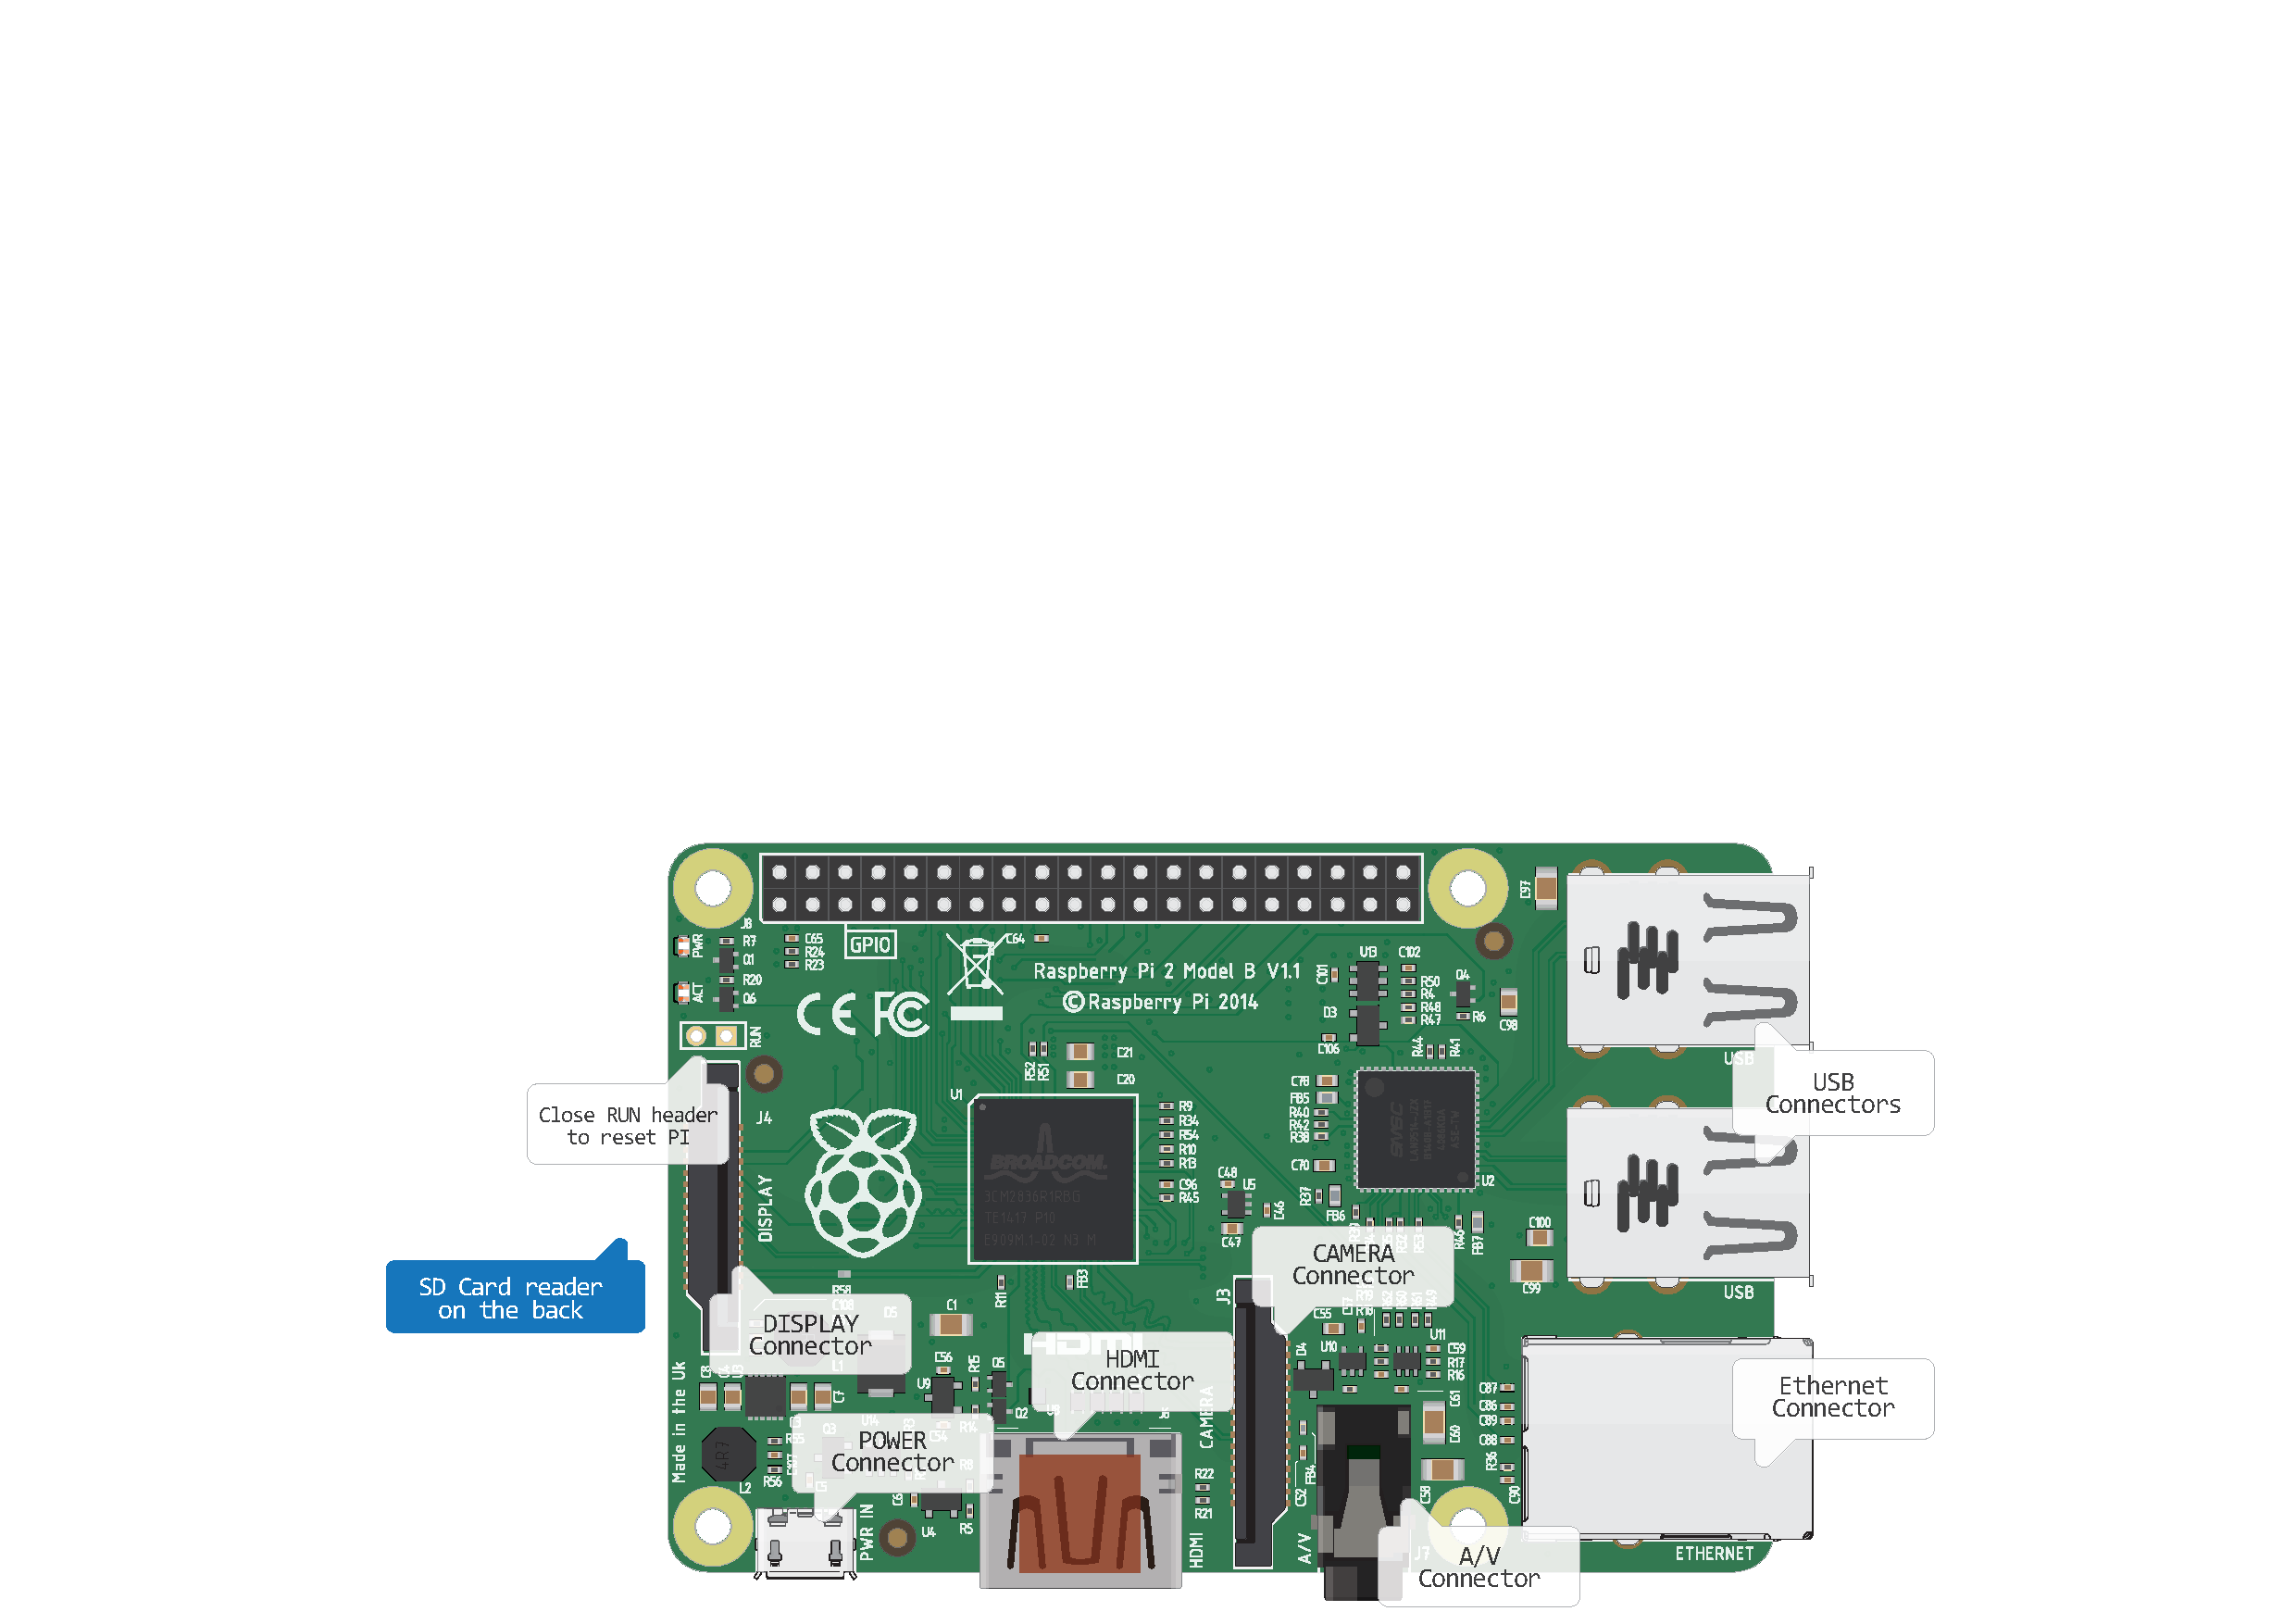
\includegraphics[width=6in]{figures/rasp.pdf}
\caption{Raspberry Pi二代B型}
\label{RASP_EPS}
\end{figure}
系统选择上,本文选择使用树莓派基金会的Debian系统,Linux内核版本为3.18\footnote{内核源码下载地址:\url{https://github.com/raspberrypi/linux}}。内核调试方案则选择使用KGDB调试工具,支持内核源码级别调试。
\subsection{Netfilter}
NC层实施方案有两种。第一种是直接在内核的TCP协议源码上更改,添加我们的NC层各个模块,然后再编译内核源码;第二种则是利用Linux内核提供给用户用于处理网络封包的框架——Netfilter,很多防火墙软件都是基于Netfilter开发的。考虑到工程复杂度,本文选择的是Netfilter框架。
\begin{figure}[htbp]
	\centering
	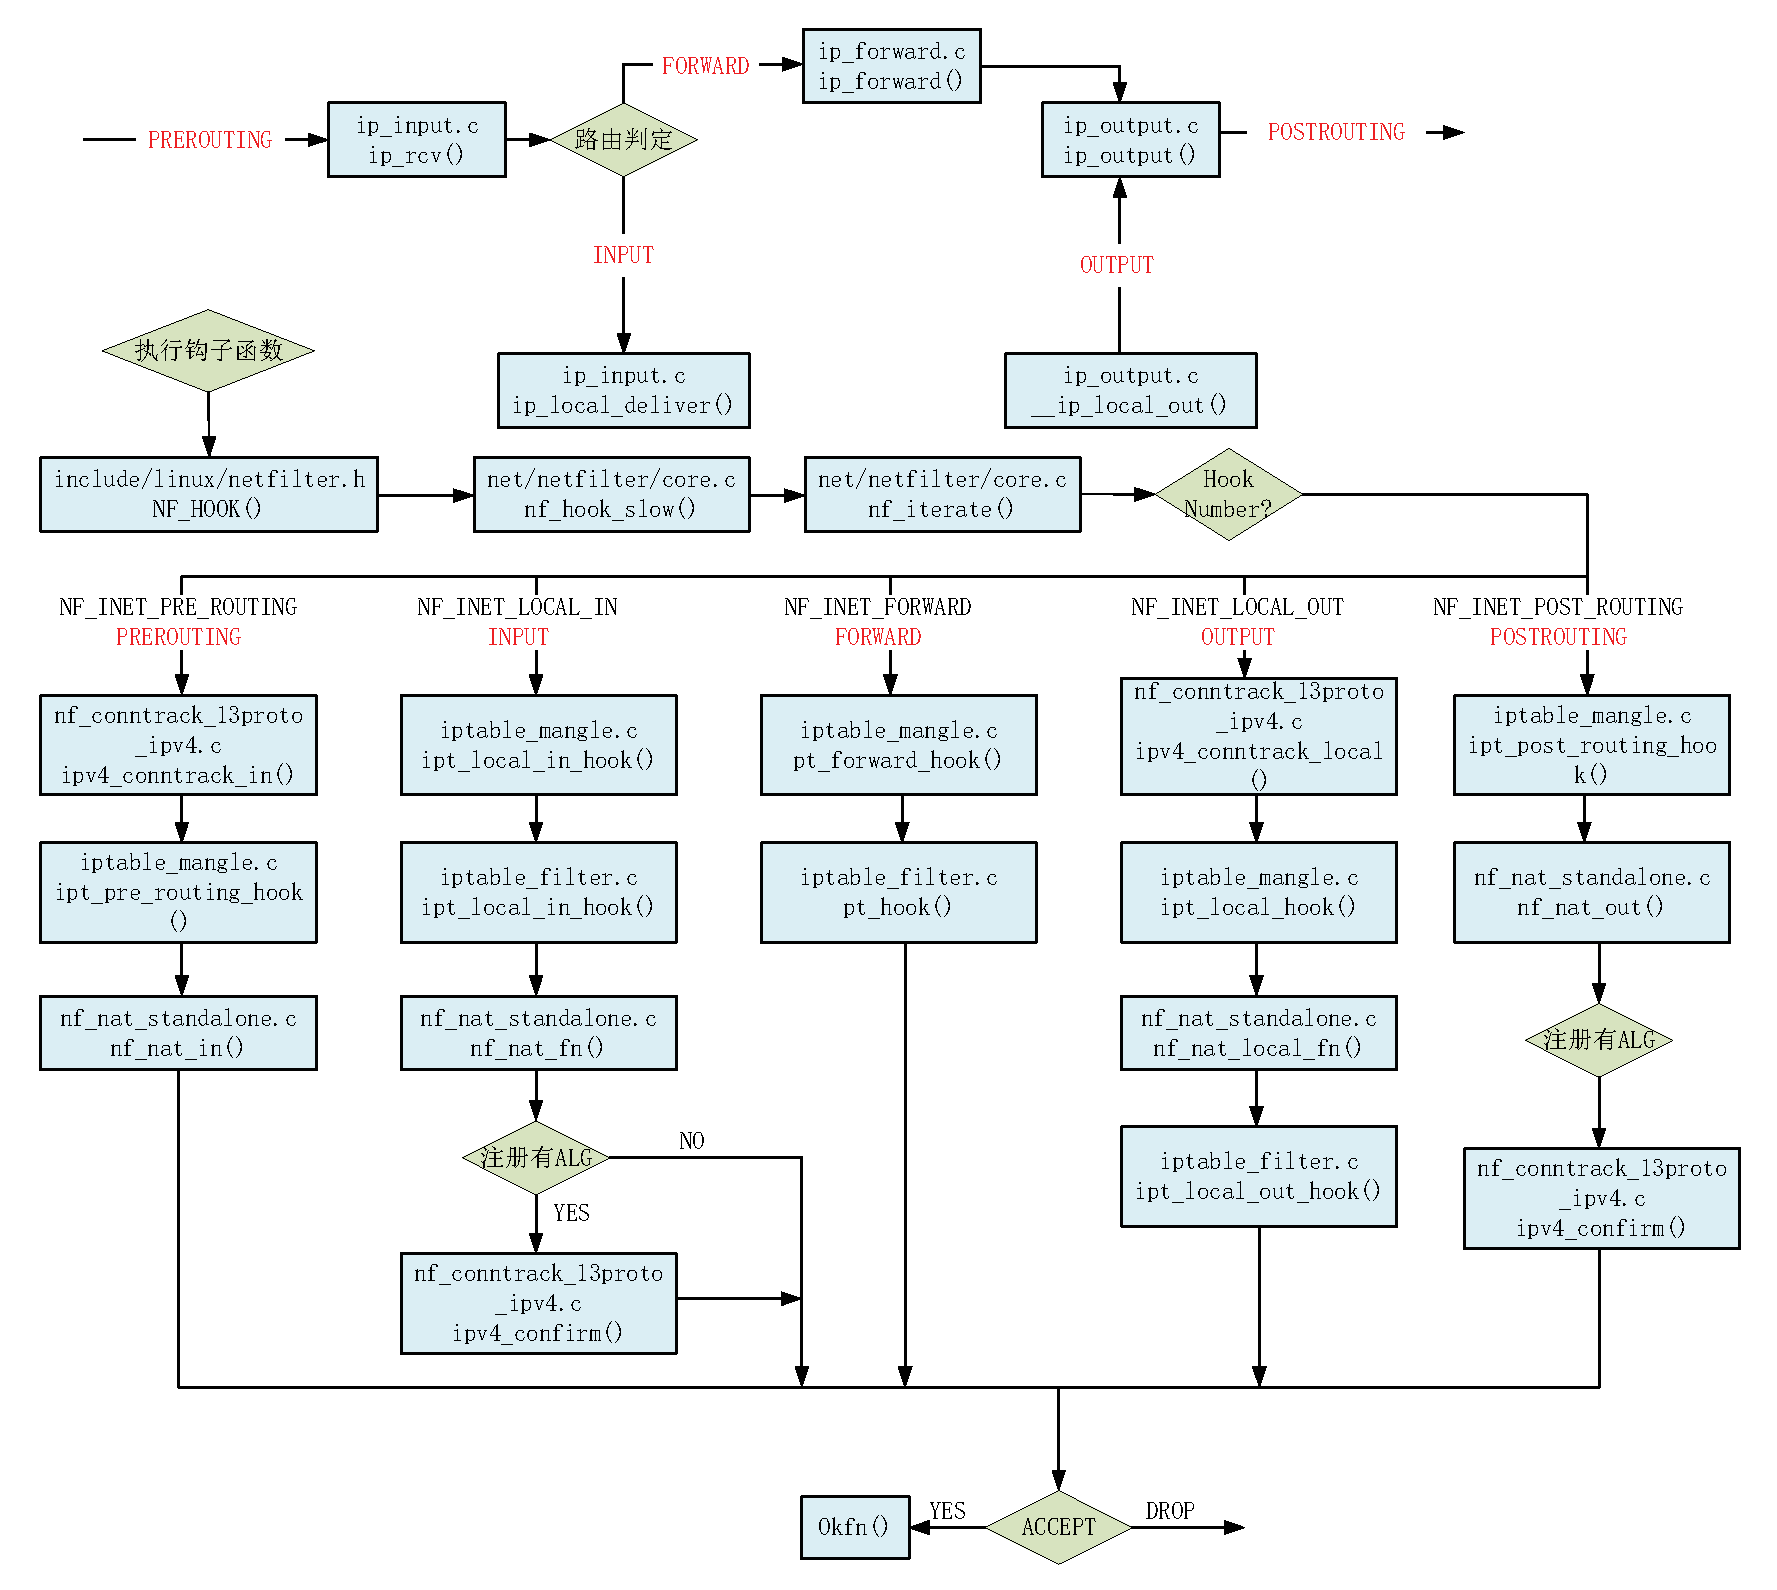
\includegraphics[width=6in]{figures/packetflow.eps}
	\caption{Netfilter框架及其在内核源码中调用关系}
	\label{NETFILTER_EPS}
\end{figure}
Linux中最常用、最基本的防火墙软件称为$iptables$。$iptables$防火墙通过与Linux内核网络协议栈的包过滤钩子交互来工作。这些内核钩子被称为Netfilter框架。Linux系统中允许注册钩子程序的点有5个。数据包在路过Linux的网络协议栈时( 出去或者进来 ) 将触发这些钩子,允许注册这些钩子的函数处理处在钩子点处的报文。数据包所触发的钩子取决于数据包是传入还是传出,数据包的目的地,以及数据包在上一个钩子点是否被丢弃或拒绝。
\par
以下钩子表示网络协议栈中有标准定义的钩子点:
\begin{itemize}[leftmargin=.5in]
	\item \textbf{NF\_IP\_PRE\_ROUTING}:数据包在进入协议栈之后,在对这个数据包作出路由决定之前,会触发这个钩子。
	\item \textbf{NF\_IP\_LOCAL\_IN}:如果一个数据包是送往本机的,那么在作出这个路由决定之后,就会触发这个钩子。
	\item \textbf{NF\_IP\_FORWARD}:如果一个数据包经过路由判定是送往其他机器的,那么就会触发这个钩子。
	\item \textbf{NF\_IP\_POST\_ROUTING}:在数据包离开本机之前,会触发这个钩子。触发这个钩子的数据包包括从本机发往网络的包和仅仅是经过本机的路由判定后发往网络中其他机器的报文。
	\item \textbf{NF\_IP\_LOCAL\_OUT}:数据包由本地发出去时,会执行挂载在这个钩子上的模块。
\end{itemize}
\par
图\ref{NETFILTER_EPS}展示的是Netfilter的框架及其在内核源码的调用关系。想要在这些钩子点注册的内核模块还需要提供一个优先级,用于决定在触发这个钩子时,按照一个什么顺序执行挂载在这些钩子上的模块。本论文的NC层就是架构于Netfilter框架,将我们的NC层编码模块分别挂在NF\_IP\_LOCAL\_IN和NF\_IP\_LOCAL\_OUT这两个钩子点上。这样我们的NC层就接管了进出本机的报文,达到了将NC层插入TCP层和IP层之间的目的。
\section{系统框架}
图\ref{JIAGOU_EPS}展示的是TCP/NC的实现架构,虚线框内的就是NC层。对于从TCP层下来的报文,首先要根据TCP报文头部信息判定是何种报文。如果是控制报文,如TCP连接建立的三次握手、RST报文,则交由控制报文处理模块进行分类处理。这些控制报文没有包含数据,无需经过编解码即可发往IP层。如果从TCP层下来的是数据报文,则需要被送到编码模块进行编码。编码后的数据包需要添加NC头部,填写NC层的控制信息,如编码包的系数、长度等。NC报文组包完毕后被发往IP层。对于从TCP层下来的纯ACK报文( 不带数据 ),也需要添加NC头部,主要是为了不浪费向对端传递NC层的相关信息的机会。
\par
从IP层上来的报文也需要经过数据包类别判定。控制报文直接交给控制报文处理模块处理,然后交给上层TCP层。对于纯ACK则在提取NC层有用信息后再交付给上层TCP层。数据报文则送到解码模块进行解码,不论解码成功,亦或是仅仅看到某个报文( see a packet ),解码模块都需要和NC层控制单元交互信息,以便让NC层控制单元决定是否向TCP连接的对方回复ACK。
\begin{figure}[htbp]
	\centering
	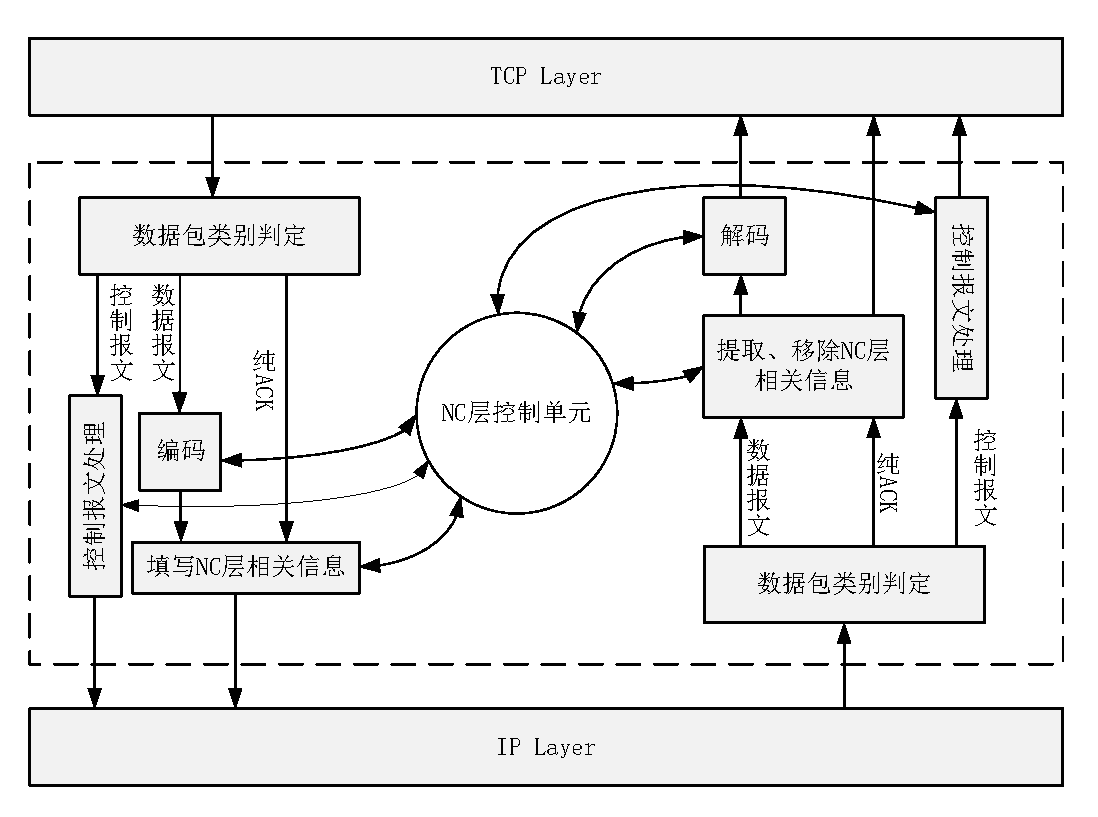
\includegraphics[width=6in]{figures/jiagou.eps}
	\caption{TCP/NC实现架构}
	\label{JIAGOU_EPS}
\end{figure}


%---------------------------------------------------------------------------------
%                西南交通大学研究生学位论文:第四章内容
%---------------------------------------------------------------------------------
\chapter{TCP/NC的改进及真实环境测试}
本章主要对文献\cite{Sundararajan2009}所提的TCP/NC给出几点改进,并加以实现,以验证相关性能。提出了前向重传机制以应对一个RTO内的突发丢包;提出了一种新的自适应冗余度算法以应对网络的变化;对冗余包的发送时机给出改进以降低平均解码时延。
\section{前向重传机制}
\subsection{TCP/NC的突发丢包问题}
通过冗余编码,TCP/NC可以很好地应对随机丢包网络的丢包。但当突发丢包发生时,TCP/NC表现就不好了。当突发丢包产生时,一般会要求重传,而TCP/NC的报文重传任务完全依赖TCP层。为了提高TCP/NC在突发丢包网络中的性能,本文提出了一种前向重传机制,能够同时高效地重传多个报文。
\par
通过增大TCP/NC的编码窗口可以提高TCP/NC应对突发丢包的能力,但是带来的后果是解码端运算复杂度的急剧增加,进而增大解码时延。在未发生超时重传时,TCP层单个、按序地在多个RTT内重传各个丢失的报文,因此TCP/NC会消耗很长一段时间来重传丢失的报文。图\ref{FR_EPS}展示了在丢了4个报文的情况下,TCP/NC是如何重传丢失的报文的。图\ref{FR_EPS}例子中设定的编码窗口值为2,冗余度为$\frac{1}{7}$,也就是说每7个编码包,多发一个冗余包。可以看到源端对$p_2$,$p_3$,$p_4$的重传总共耗费了3个RTT,导致目的端的NC层虽然在收到$C\left[8\right]$时就开始可以解码$p_5$后面的报文,但由于乱序,无法将它们上交给上层的TCP。
\par
在TCP-Reno中,对于重复ACK采取的是快速重传的方法。以图\ref{FR_EPS}为例,源端的NC层在收到3个对$p_2$的ACK之后,直接将其交付给上层TCP。上层TCP收到3个重复的对$p_2$的ACK,认为报文$p_2$丢失了,采取快速重传,只重传$p_2$,然后进入拥塞避免阶段,继续接着$p_{10}$发送$p_{11}$。接收端在收到$p_2$的重传报文$C\left[11\right]$后,又陆续回给源端多个重复ACK,表示$p_3$丢失。源端TCP又启动快速重传,重传报文$p_3$。后面对报文$p_4$的重传和$p_1$,$p_2$的情况一样。当编码窗口的值更大,RTT比较大时,这种情况产生的影响更大。
\par
TCP-Reno对于一个RTO内报文的连续丢失采取的是单个依次重传的处理策略,因此对突发丢包不是很友好。NC层的引入让这一策略的劣势更为凸显。当NC层出现重复ACK时,意味着链路中出现的丢包就绝不仅仅是单个报文的丢失,这是由于NC层的“seen”机制导致的。直觉上,由于NC层缓存有未被确认的数据包,我们可以在NC层重传那些未被看到的报文。当NC层收到第一个从TCP层下来的重传报文\emph{pkt}后,NC层不仅重传\emph{pkt},而是会在一个RTT内顺便将所有未看到的报文都重传。如此,可以让上层TCP认为仅仅就丢了一个包。如图\ref{NEWFR_EPS}所示,NC层收到上层TCP的重传报文$p_2$后,在一个RTT内重传了未看到的报文$p_2$,$p_3$和$p_4$。
\begin{figure}[htbp]
	\centering
	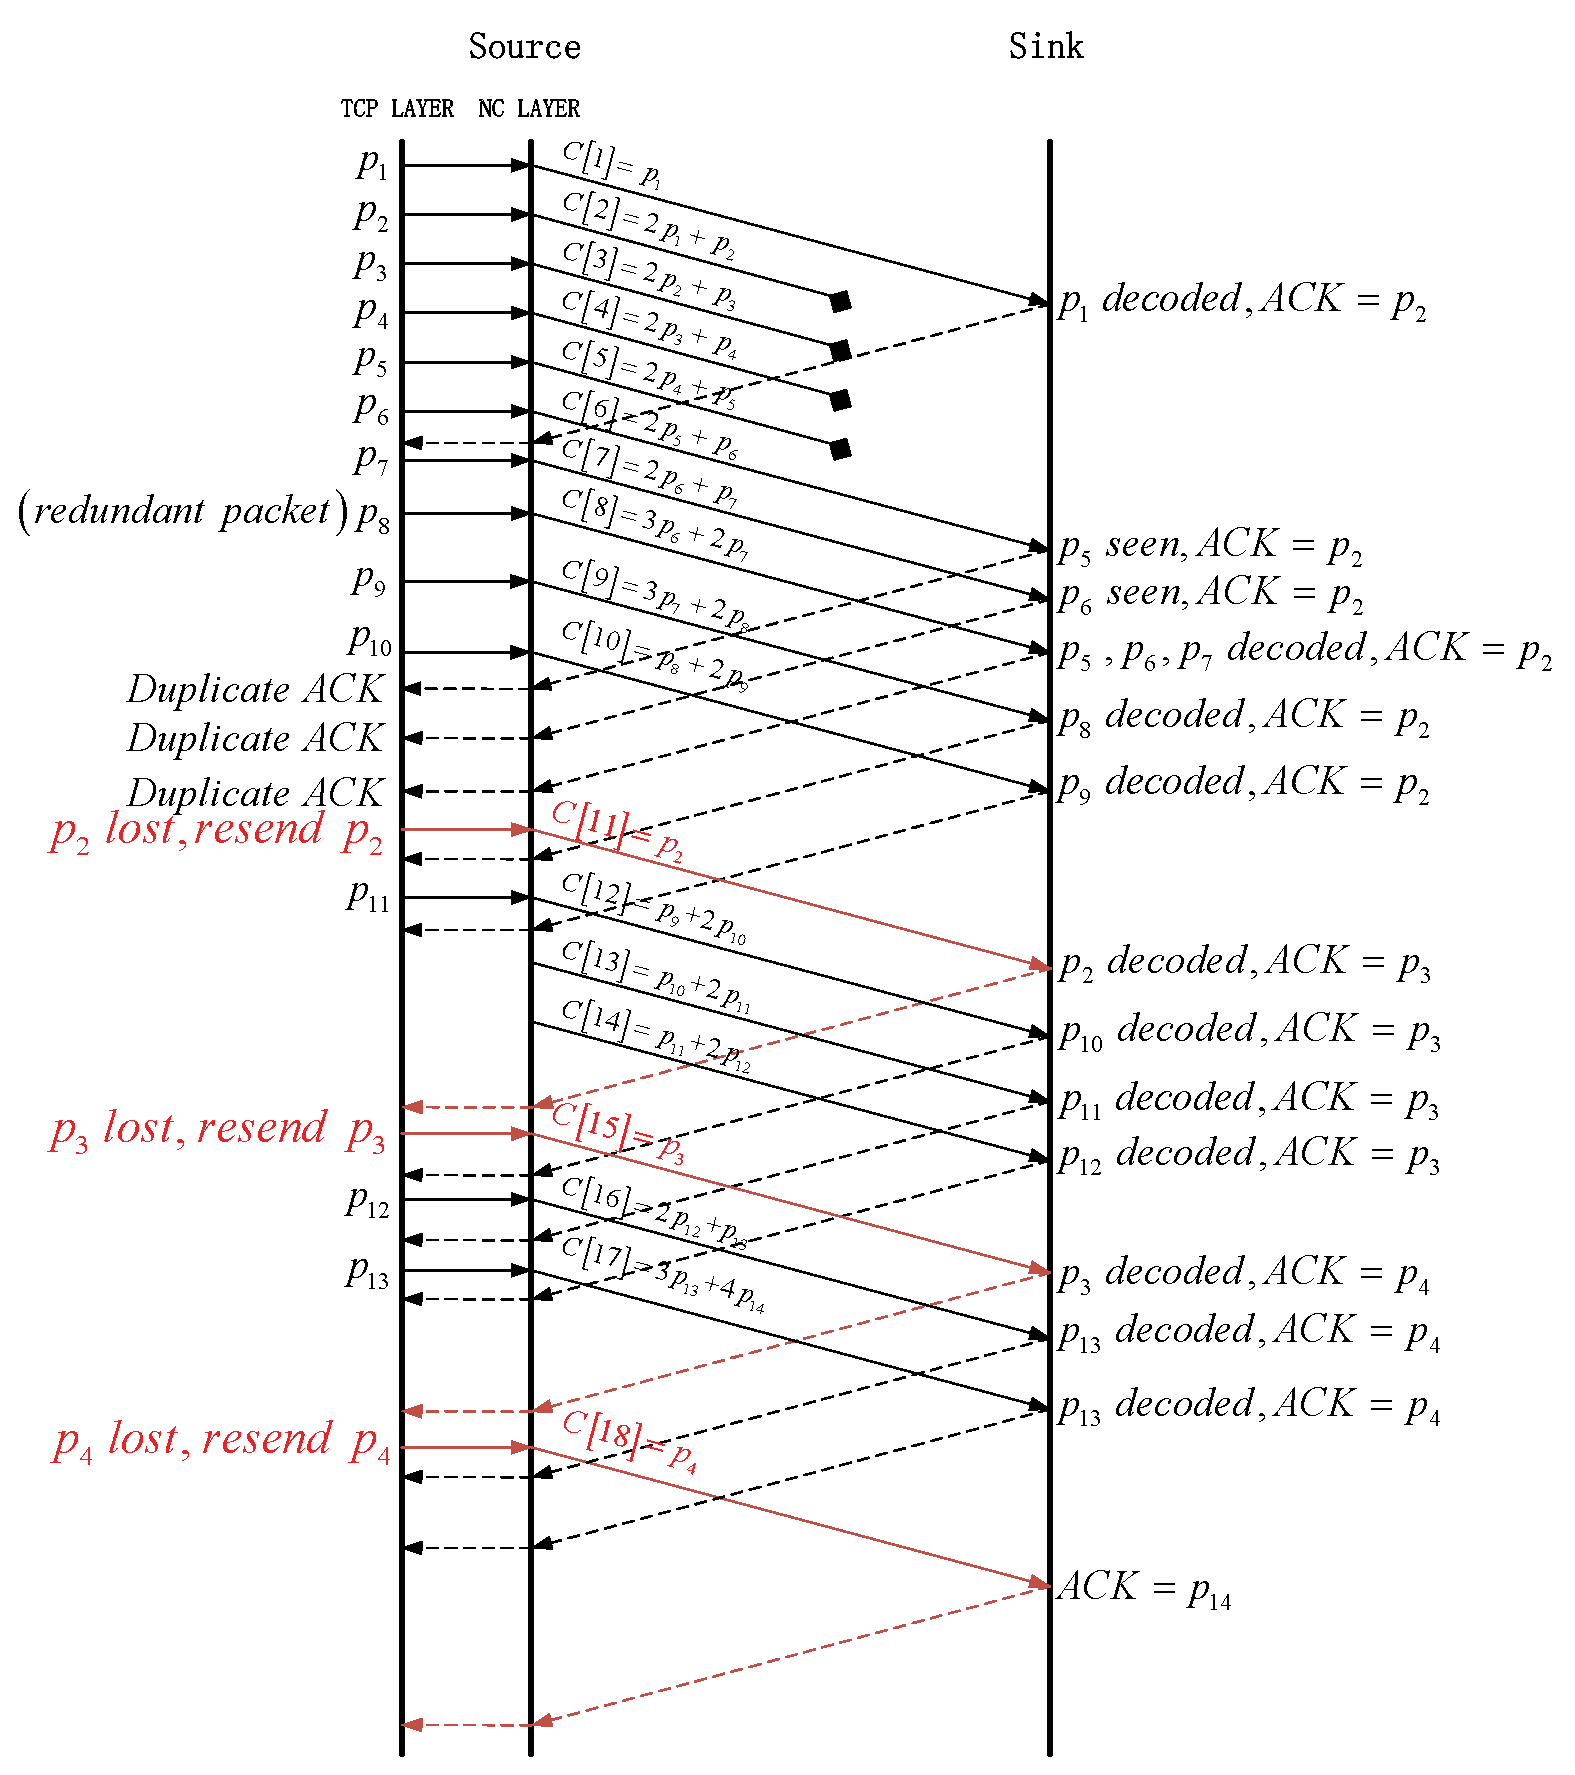
\includegraphics[width=4in]{figures/fr.eps}
	\caption{原有TCP/NC的重传机制}
	\label{FR_EPS}
\end{figure}
\begin{figure}
	\centering
	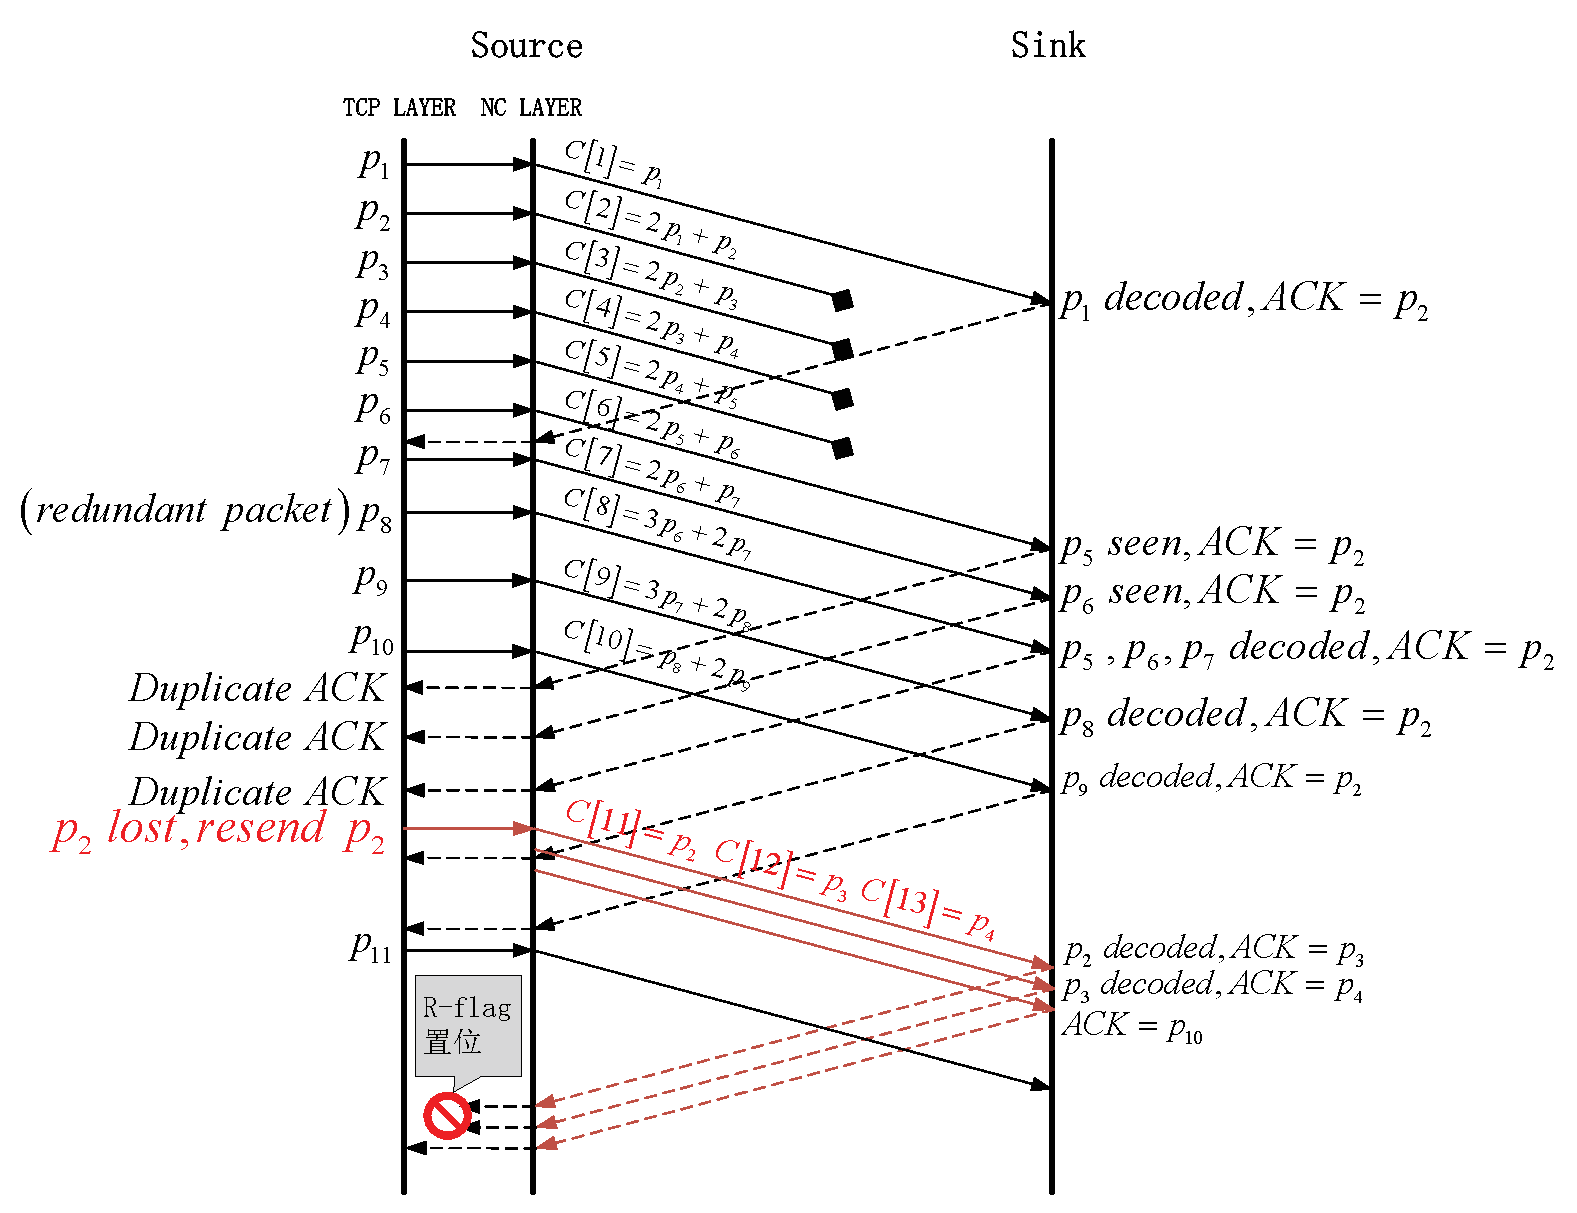
\includegraphics[width=4in]{figures/newfr.eps}
	\caption{前向重传机制}
	\label{NEWFR_EPS}
\end{figure}
\subsection{新NC头部设计}
为了支撑前向重传机制,本文设计了新的NC头部,如图\ref{NEWHEADER_EPS}。原有TCP/NC头部设计 ( 图\ref{CODINGHEADER_EPS} )中的Res字段,有6个比特可供使用,对应图\ref{NEWHEADER_EPS}中的$b_1 \sim b_6$。此六个比特与标准TCP中的保留字段对应。在第\ref{ztlc}小节中,我们讲到需要区分NC报文和普通TCP报文,可以利用$b_1$标识这个是TCP报文还是NC报文。利用$b_2$表示R-flag,表示当前这个报文是否要被上交给TCP层;利用$b_3$、$b_4$和$b_5$一起表示当前报文的\emph{报文状态}( 后面会讲到\emph{报文状态}的作用 )。增加了Pid和Pid-reply两个域,各自两个字节。其中Pid表示NC层发出的报文编号,以报文为计数单位,而非字节。NC层发出的每个线性组合报文有独一无二的Pid( 回环问题另做考虑 ),接收端在收到编号为Pid的线性组合报文后,在回复的ACK报文中,Pid-reply域就填上Pid,表示当前这个ACK是由编号为Pid的线性组合包激发的。
\begin{figure}[htbp]
	\centering
	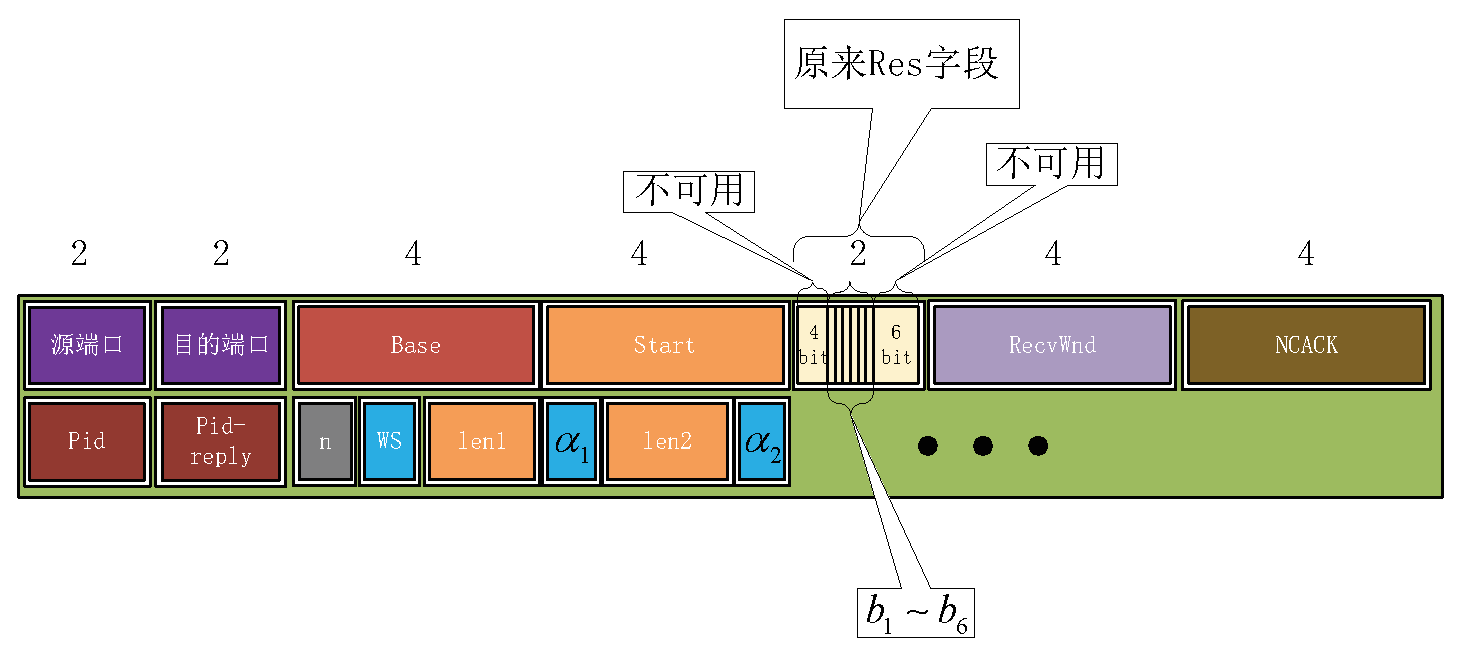
\includegraphics[width=6in]{figures/newheader.eps}
	\caption{新NC头部设计}
	\label{NEWHEADER_EPS}
\end{figure}
\subsection{定位丢包}
为了在NC层重传未被看到的报文,首先需要确定丢了哪些报文。
\par
源端保存了每个编码包的原始数据包信息,即这个编码包是由哪几个原始数据包组成的,如图\ref{FR_EPS}中的$C\left[9\right]$由$p_7$和$p_8$组成。当发送端收到接收端回复的ACK报文时,有如下几种情形。
\begin{enumerate}[fullwidth,itemindent=2em,label=(\arabic*)]
	\item 有新的数据被确认且ACK报文中R-flag( 后面会解释R-flag含义 )未置位,那么将其交给上层TCP。
	\item 有新的数据被确认而ACK报文中R-flag置位,此ACK需要被抑制,不会被交付给上层TCP,如图\ref{NEWFR_EPS}中对$C\left[11\right]$和$C\left[12\right]$的ACK,但会更新NC层中未被看到的报文,从未被看到的报文列表中移除本次新确认的数据。
	\item 本次ACK并没有确认新的数据,提取其中的\emph{Pid-reply}域,然后罗列Pid值为Pid-reply的编码包的所有原始数据包$p_i \sim p_j(i \le j)$。如果目前在发送端未被确认的数据包中最小序号为$seq_1$,$p_i$数据包的起始序号是$seq_2$,那么我们可知接收端那边未看到的报文序号是在$seq_1 \sim \left(seq_2 - 1\right)$之间。由于发送端可能会收到接收端多个这样的ACK报文,如图\ref{NEWFR_EPS}中对$C\left[6\right]$,$C\left[7\right]$和$C\left[8\right]$的确认ACK报文,未看到的报文区间会被更新,但更新的方式只能是区间长度变小,也就是说$seq_2-1$只能向着$seq_1$靠拢。以图\ref{NEWFR_EPS}为例,发送端在收到对$C\left[7\right]$的ACK后,未看到的报文区间不会改变,依然是$seq_{p_2} \sim seq_{p_5} - 1$。
\end{enumerate}
\par
从图\ref{NEWFR_EPS}中可以看到,接收端发出的对报文$C\left[11\right]$和$C\left[12\right]$的确认ACK报文被发送端的NC层抑制了,并没有交给上层。发送端的NC层直到收到ACK为$p_{10}$的报文,才将此ACK上交给上层TCP。这样达到了让上层TCP以为仅仅丢了一个包的目的。因此,我们需要在NC头部添加\emph{报文状态}字段。可以告知接收端当前这个报文能否让接收端产生确认所有重传报文的ACK报文。如果可以,那么接收端在回复给发送端的ACK报文中会将R-flag清掉;如果不行,接收端在回复给发送端的ACK报文中会对R-flag置位。这样发送端的NC层就可以根据R-flag状态来决定是否将ACK报文送往上层TCP。表\ref{tab:BWZT}展示的是所有的报文状态信息。

\begin{table}[htp]
	\centering
	\caption{报文状态描述}
	\label{tab:BWZT}
	\begin{tabular}{l|l}
		\toprule
		报文状态( $b_3b_4b_5$) &描述\tabularnewline
		\midrule
		000		& 正常的编码包\tabularnewline
		001		& 冗余编码包 \tabularnewline
		010		& 未编码重传报文,但不是最后一个\tabularnewline
		011 	& 未编码重传报文,且是最后一个\tabularnewline
		100		& 重传编码报文,但不是最后一个\tabularnewline
		101		& 重传编码报文,且是最后一个\tabularnewline
		\bottomrule
	\end{tabular}
\end{table}
\subsection{重传丢包}
每当NC层收到上层TCP下来的重传报文时,我们的前向重传机制才会启动。发送端的NC层维护了一个链表\emph{re\_list},保存着接收端那边未看到的报文;\emph{re\_list}通过接收端那边回的ACK报文来更新。是否启动前向重传取决于\emph{re\_list}是否为空。当NC层完成前向重传后,\emph{re\_list}会被清空。
\par
值得注意的是,在重传过程中,对于\emph{re\_list}中的报文,我们发送的是原始数据包,例如图\ref{NEWFR_EPS}中的$p_2$、$p_3$和$p_4$。这是为了加快接收端的解码进程。对照表\ref{tab:BWZT},图\ref{NEWFR_EPS}中报文$p_2$和$p_3$的\emph{报文状态}域上填写的都是010;报文$p_4$的\emph{报文状态}域上填写的是011。这是由于$p_4$是这个非编码重传序列的最后一个重传报文。接收端在收到重传的$p_2$、$p_3$和$p_4$后会产生3个ACK报文,通过检查$p_2$、$p_3$和$p_4$的\emph{报文状态}域,接收端知道$p_4$才是这个非编码重传序列的最后一个重传报文。因此,对于$p_2$、$p_3$的ACK报文,接收端会对其R-flag域置位,让发送端的NC层不将$p_2$和$p_3$的ACK报文上传给TCP层;而对于$p_4$的ACK报文,接收端会清掉R-flag域,让发送端的NC层将$p_4$的ACK报文上传给TCP层。
\par
考虑一下重传报文丢失的情况。
\begin{enumerate}[fullwidth,itemindent=2em,label=(\arabic*)]
	\item 如果重传序列的第一个报文或者中间报文丢失,那么依然会触发重复ACK,情形退回到前向重传机制开始之前的情况。
	\item 如果最后一个重传报文,如$p_4$丢失,那么发送端只会收到R-flag置位的ACK报文,如$p_2$和$p_3$的ACK报文;由于R-flag置位,发送端的NC层不会将这些ACK报文上交给TCP层,但是会更新NC层的编码缓存;一段时间后上层TCP会重传刚刚才重传过的报文序列,如$p_2$、$p_3$和$p_4$;NC层发现$p_2$和$p_3$被接收端确认了,会立马创建一个ACK报文,回给上层TCP;NC层发现\emph{re\_list}为空,$p_4$不在\emph{re\_list}中,而$p_4$在编码缓存中,因此会将$p_4$加入到\emph{re\_list},重传$p_4$,并清空\emph{re\_list}。
\end{enumerate}
\par
考虑一下超时重传的情况。NC层通过检查TCP层下来的报文是否在编码缓存中来确定这个报文是否是重传包。不管是超时重传报文还是快速重传报文,都首先检查该报文是否在\emph{re\_list}中,如果不在就加入到\emph{re\_list},然后重传\emph{re\_list}的所有报文。
\subsection{编码重传包}
考虑到重传序列的最后一个重传包丢失造成的性能损失比较大,本文对重传报文进行再编码。在重传了\emph{re\_list}的所有不编码原始报文后,再重传$\left\lceil {R \times num\_re} \right\rceil  - num\_re$个编码报文,其中\emph{R}表示冗余度,\emph{num\_re}表示\emph{re\_list}中重传报文的个数。重传编码报文的\emph{报文状态}域填写方式参照表\ref{tab:BWZT}。
\section{改进冗余包发送时机}
文献\cite{Sundararajan2009}中冗余包分布并非均匀分布。给定一个固定冗余度,其冗余特性并没有体现在每个编码包中。因此本文重新设计了冗余包的发送时机。假定冗余度为\emph{R} ( $R \ge 1$ ),对于从TCP层下来的每个报文,以$R - \left\lfloor R \right\rfloor$的概率发送 $\left\lfloor R+1 \right\rfloor$个编码包;以$1-\left(R-\left\lfloor R \right\rfloor\right)$的概率发送$\left\lfloor R \right\rfloor$个编码包。这样冗余度均匀分布在每个数据包中了。
\section{自适应冗余度算法}
文献\cite{Sundararajan2009}中并没有给出冗余因子\emph{R}的设置规则。自觉告诉我们,将\emph{R}设置为一个常量值是不合适的。现实中的网络环境,尤其是无线环境,其丢包率是在变动的。在设置冗余因子时,如果\emph{R}过小,那么冗余信息不足以掩盖链路中的丢包;如果\emph{R}值过大,编码码率就过小,降低网络的有效吞吐率。因此需要找出一种能够根据网络状况自适应调整冗余度的方法,最大化地利用网络带宽。
\par
文献\cite{6261883}针对TCP/NC提出了一种自适应冗余算法。作者借鉴TCP-Vegas中的\emph{Vegas loss predictor}\textsuperscript{\cite{martignon2004loss,brakmo1995tcp}},在NC层实现了一个\emph{loss differentiation scheme}。通过估计当前的网络拥塞状态和收到的重复ACK信息,在让网络不出现拥塞的前提下可以动态调整冗余度。其缺点则是\emph{Vegas loss predictor}在面对TCP-Reno竞争时的无力\textsuperscript{\cite{hasegawa2000fairness}}。
\par
文献\cite{song2011self}设计了SANC-TCP,其基本思想是对产生的编码报文进行编号,在ACK的头部添加两个域\emph{loss}和\emph{echo\_pktID}。发送端根据接收到的ACK报文中的\emph{loss}和\emph{echo\_pktID},以及编码窗口的值来动态调整冗余度。其中\emph{loss}表示接收端的解码矩阵中序号最大的原始数据包编号和“seen packets”编号之间的差值;\emph{echo\_pktID}表示哪个报文激发了本次ACK。其在调整冗余度时不仅考虑了当前网络的丢包率,还将接收端的解码矩阵的状态信息考虑进去。
\par
考虑到在设计前向重传机制中引入的Pid和Pid-reply字段,本文依据Pid和Pid-reply设计了一个新的自适应冗余算法。由文献\cite{Sundararajan2011}中可知,冗余度\emph{R}与丢包率密$\rho$密切相关,理想情况下其关系为
\begin{equation}
	R=\dfrac{1}{1-\rho}
\end{equation}
因此需要知道当前链路的丢包率。可以由Pid和Pid-reply字段计算得到。如图\ref{DIUBAO_EPS}中展示,发送端提取接收到的ACK中的Pid-reply字段即可了解Pid=103的报文丢失了,进而计算在Pid=100到Pid=104时段内的丢包率$\rho=25\%$。需要注意如下几点:
\begin{itemize}[leftmargin=.5in]
	\item 对于每个编码包包都会回复ACK
\end{itemize}
\begin{figure}[htbp]
	\centering
	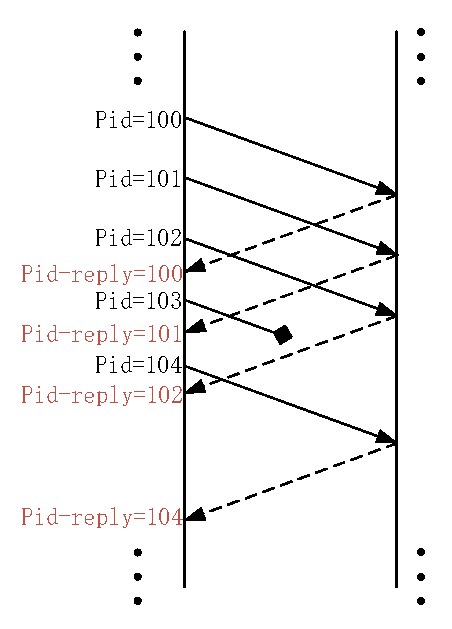
\includegraphics[width=3in]{figures/diubao.eps}
	\caption{计算丢包率示例}
	\label{DIUBAO_EPS}
\end{figure}
\section{反馈重传算法}
\section{真实网络环境测试}
\subsection{无人机lossy信道环境搭建}
\subsection{测试结果}
\subsection{性能分析}
\section{本章小结}
为了在真实丢包环境中测试TCP/NC及其改进协议的性能,本文搭建了无人机测试环境。将部署了TCP/NC改进协议的Raspberry Pi搭载在无人机上,通过WIFI无线链路来与地面站通信。 
%\chapter{论文工作总结与展望}

% 加载论文结论
%---------------------------------------------------------------------------------
%                西南交通大学研究生学位论文:结论
%---------------------------------------------------------------------------------
\chapter*{结\qquad{}论}
\addcontentsline{toc}{chapter}{结论}
本章将对本论文的工作进行总结,
并对后续进一步的研究问题进行讨论。
\section*{本文工作总结}
随着集成电路技术、通讯技术的飞速发展,
无人机航拍逐渐成了普通人都可以应用的一项技术。
由于设备价格低廉、未来5G时代万物互联的前景,
基于现有TCP/IP协议栈体系的无人机视频传输技术仍然具有很大前景。
由于无人机工作于室外空域,
面临的是典型的大尺度衰落信道环境,
丢包、错包频繁,
面向有线网络设计的标准TCP无法很好应对这种场景,
导致无人机视频传输吞吐率上不去、时延很大。
\par
本文首先分析了基于TCP协议的无人机视频传输所面临的问题,
查阅了大量文献,总结了前人做出的关于提高TCP在有损信道环境下的表现的工作。
重点分析论述了Sundararajan等人的工作,即TCP/NC。
在Raspberry Pi上实现了TCP/NC协议,
并对TCP/NC在有损信道环境下的表现做了测试、分析。
与前人工作不同的是,
在详细比较了Batch Coding和Pipeline Coding的优缺点后,
根据TCP协议的滑动窗口概念,
采用了Pipeline Coding编码方式实现网络编码。
\par
针对TCP/NC在无人机视频传输应用场景中所存在的问题,
本文对其做了进一步改进,实现增强TCP/NC协议,即E-TCP/NC。
提出了前向重传机制以应对一个RTO内的突发丢包;
提出了一种新的自适应冗余度算法以应对网络的变化;
对冗余包的发送时机给出改进以降低平均解码时延;
设计补偿重传机制以降低解码端解码矩阵维度和减小解码时延;
改进编码系数的设定以降低首部开销。
最后本文搭建了无人机视频传输实验平台,
测试E-TCP/NC对无人机视频传输性能的提升。

\section*{未来工作展望}
在下一步的研究和学习过程中,我们将在以下方面做出改进:
\begin{enumerate}[fullwidth,itemindent=2em,label=(\arabic*)]
	\item NC层的编解码过程耗费资源太大。
	如第\ref{sec:monidiubaoceshijieguo}小节所述,
	100M网卡在添加了编解码模块后,
	峰值速度直接降到了12Mbps。
	这其中有代码优化原因,
	也有Raspberry Pi性能有限的原因,
	但本质上是由于编解码本来就耗费资源,
	而本文又以模块的形式实现E-TCP/NC,
	导致软中断时间过长,
	影响最终吞吐率。
	在今后的工作中,
	将优化目前代码,
	寻求新的编解码方式,
	以便可以同时处理多个字节,
	降低解码端的开销。
	\item 目前对TCP报文的处理仅仅覆盖了一部分情况,
	对于TCP协议的选项字段、URG字段、PSH字段等都未做处理。
	后期需要改进目前的实现,
	使E-TCP/NC完全兼容目前的TCP协议。
	\item TCP中对ACK反馈的依赖加大了无人机视频传输的时延,
	目前有学者已经做出了相关工作\textsuperscript{\cite{ontheflycoding}},
	降低TCP对ACK的依赖,
	后期的工作中,
	将尝试将其与E-TCP/NC结合起来。
\end{enumerate}

%---------------------------------------------------------------------------------
% 论文附录(包括致谢、参考文献、证明、工作列表)

% 加载致谢文件
%---------------------------------------------------------------------------------
%                西南交通大学研究生学位论文:致谢
%---------------------------------------------------------------------------------
\chapter*{致\qquad{}谢}
\addcontentsline{toc}{chapter}{致谢}

在西南交通大学研究生学位论文~\LaTeX{}~模板swjtuThesis的开发制作过程中,主要参考了以下的国内高校学位论文~\LaTeX{}~模板,在此对所有的模板作者表示由衷的感谢:
\begin{compactitem}
	\item 中国科大学位论文通用~\LaTeX{}~模板(目前为数不多经过校方认证发布的模板)\footnote{下载地址:\url{http://gradschool.ustc.edu.cn/ylb/material/xw/wdxz.html}}
	\item 清华大学学位论文~\LaTeX{}~模板~thuthesis\footnote{下载地址:\url{https://github.com/xueruini/thuthesis}}
	\item 北京大学学位论文~\LaTeX{}~模板~pkuthss\footnote{下载地址:\url{https://github.com/CasperVector/pkuthss}}
	\item 浙江大学研究生硕士(博士)学位论文~\LaTeX{}~模板\footnote{下载地址:\url{https://github.com/ZJU-Awesome/write_with_LaTeX}}
	\item 哈工大硕博士毕业论文~\XeLaTeX{}~模版~PlutoThesis\footnote{下载地址:\url{https://github.com/dustincys/PlutoThesis/releases}}
	\item 南京理工大学学位论文~\LaTeX{}~模版\footnote{下载地址:\url{https://github.com/jiec827/njustThesis}}
	\item 北京交通大学毕设~\LaTeX{}~模板~bjtuThesis\footnote{下载地址:\url{https://github.com/chenzewei01/bjtuThesis}}
\end{compactitem}

\par
最后,感谢所有在swjtuThesis模板开发过程中予以了各种无私帮助的老师和同学。其中特别感谢:西南交通大学电气工程学院智能牵引供电团队胡海涛副教授在模板开发过程中提出的若干意见,博士研究生杨鸣凯对模板基于CTeX端的调试;交通运输与物流学院14级硕士研究生甘婧对模板存在的一些问题的指正;此外还有西南交通大学博士研究生冯玎、王玘、王湘、李勇,硕士研究生张佳怡等,在此一并感谢。

\par
希望未来能有更多的同学加入学位论文文~\LaTeX{}~模板的开发和完善工作,推广~\LaTeX{}~在国内青年学生学者圈子中使用。

\vspace{25mm}
\begin{flushright}
	原始作者:Limin HUANG \\
	@ Studio0513
\end{flushright}

% 加载参考文献
\bibliographystyle{ref/chinesebst}			% 定义参考文献列表格式,参考国标文件GB/T 7714-2015制作
%%\bibliography{ref/refEx}					% 加入参考文献的.bib库,可自行建立替换,refEx为示范文件
\bibliography{ref/refs}
\addcontentsline{toc}{chapter}{参考文献}

% 加载附录文件和个人工作列表
%%---------------------------------------------------------------------------------
%                西南交通大学研究生学位论文:附录A
%---------------------------------------------------------------------------------
% 附录部分的可操作性很强,可以是部分测试数据、数学证明或者是个人简介,请根据需求修改
\chapter*{附录~A}							% 附录环节属于无编号章节
\addcontentsline{toc}{chapter}{附录~A}	% 定义字符串,把无编号章节加入目录中(如附录A)						% 非必要章节,主要用以放置测试数据、数学证明或者个人简介
%---------------------------------------------------------------------------------
%                西南交通大学研究生学位论文:所取得的科研成果
%---------------------------------------------------------------------------------
\chapter*{攻读\cDegree{}学位期间发表的论文及科研成果}
\addcontentsline{toc}{chapter}{攻读\cDegree{}学位期间发表的论文及科研成果}

\section*{1.~发表学术论文}
\begin{publist}
	\item \textbf{姜维}, 诸葛亮, 赵云, 等. 基于战争大数据的九伐中原与六出祁山的战略决策分析[J]. 中国战争信息物理, 2015, 40(13): 520-530.(SCI~收录号: , IF=0.16)
	\item \textbf{姜维}, 诸葛亮, 刘禅, 等. 基于神经网络的子午谷奇谋仿真研究[J]. 战争仿真学报, 2015, 19(4): 324-330.(EI~收录号:)
	\item W. Jiang, G. L. Zhu. , et al. Improved $\mathcal{H}_\infty$ Robust Control Design for Mu-Niu-Liu-Ma System[C]. Intelligent System Design and Applications, Chengdu, 2015. EI~收录号:)
\end{publist}

\section*{2.~申请国家专利}
\begin{publist}
	\item 诸葛亮, \textbf{姜维}. 一种木牛流马的制造方式及其使用方法. 中国, 20152006387.1[P]. xxxx-xx-xx.
\end{publist}

\section*{3.~参与科研项目}
\begin{publist}
	\item \textbf{学生第一主研}, 高效粮食载运工具基础科学问题研究与样机研制, 蜀自然科学基金项目. 课题编号: XXXX.
\end{publist}					% 攻读硕(博)士论文攻读期间取得的科研成果,论文、专利等

\end{document}